%%%%%%%%%%%%%%%%%%%%%%%%%%%%%%%%%%%%%%%%%%%%%%%%%%%%%%%%%%%%%%%%%%%%
%% I, the copyright holder of this work, release this of into the
%% public domain. This applies worldwide. In some countries this may
%% not be legally possible; if so: I grant anyone the right to use
%% this work for any purpose, without any conditions, unless such
%% conditions are required by law.
%%%%%%%%%%%%%%%%%%%%%%%%%%%%%%%%%%%%%%%%%%%%%%%%%%%%%%%%%%%%%%%%%%%%

\documentclass[
  print, %% This option enables the default options for the
           %% digital version of a document. Replace with `printed`
           %% to enable the default options for the printed version
           %% of a document.
  table,   %% Causes the coloring of tables. Replace with `notable`
           %% to restore plain tables.
  nolof,     %% Prints the List of Figures. Replace with `nolof` to
           %% hide the List of Figures.
  nolot,     %% Prints the List of Tables. Replace with `nolot` to
           %% hide the List of Tables.
           %draft, %TODO remove, place final instead
           oneside
  %% More options are listed in the user guide at
  %% <http://mirrors.ctan.org/macros/latex/contrib/fithesis/guide/mu/fi.pdf>.
]{fithesis3}
%% The following section sets up the locales used in the thesis.
\usepackage[resetfonts]{cmap} %% We need to load the T2A font encoding
\usepackage[T1,T2A]{fontenc}  %% to use the Cyrillic fonts with Russian texts.
\usepackage[
  main=english, %% By using `czech` or `slovak` as the main locale
                %% instead of `english`, you can typeset the thesis
                %% in either Czech or Slovak, respectively.
  %german, russian, czech, slovak %% The additional keys allow
]{babel}        %% foreign texts to be typeset as follows:
%%
%%   \begin{otherlanguage}{german}  ... \end{otherlanguage}
%%   \begin{otherlanguage}{russian} ... \end{otherlanguage}
%%   \begin{otherlanguage}{czech}   ... \end{otherlanguage}
%%   \begin{otherlanguage}{slovak}  ... \end{otherlanguage}
%%
%% For non-Latin scripts, it may be necessary to load additional
%% fonts:
\usepackage{paratype}
\def\textrussian#1{{\usefont{T2A}{PTSerif-TLF}{m}{rm}#1}}
%%
%% The following section sets up the metadata of the thesis.
\thesissetup{
    date          = \the\year/\the\month/\the\day,
    university    = mu,
    faculty       = fi,
    type          = mgr,
    author        = Lukáš Němec,
    gender        = m,
    advisor       = {RNDr. Petr Švenda, Ph.D.},
    title         = {Edu-hoc: Experimental and educational platform for wireless ad-hoc networking},
    TeXtitle      = {Edu-hoc: Experimental and educational platform for wireless ad-hoc networking},
    keywords      = {keyword1, keyword2, ...},
    TeXkeywords   = {keyword1, keyword2, \ldots},
}
\thesislong{abstract}{
    TODO abstract
}
\thesislong{thanks}{
    TODO thanks

}
%% The following section sets up the bibliography.
\usepackage{csquotes}
\usepackage[              %% When typesetting the bibliography, the
  backend=biber,          %% `numeric` style will be used for the
  style=numeric,          %% entries and the `numeric-comp` style
  citestyle=numeric-comp, %% for the references to the entries. The
  sorting=none,           %% entries will be sorted in cite order.
  sortlocale=auto         %% For more unformation about the available
]{biblatex}               %% `style`s and `citestyles`, see:
%% <http://mirrors.ctan.org/macros/latex/contrib/biblatex/doc/biblatex.pdf>.
\addbibresource{bibliography.bib} %% The bibliograpic database within
                          %% the file `example.bib` will be used.
\usepackage{makeidx}      %% The `makeidx` package contains
\makeindex                %% helper commands for index typesetting.
%% These additional packages are used within the document:
\usepackage{paralist}
\usepackage{amsmath}
\usepackage{amsthm}
\usepackage{amsfonts}
\usepackage{url}
\usepackage{menukeys}


\usepackage{wrapfig}

\begin{document}


%% We will define several mathematical sectioning commands.
%\newtheorem{theorem}{Theorem}[section] %% The numbering of theorems
                               %% will be reset after each section.
%\newtheorem{lemma}[theorem]{Lemma}     %% The numbering of lemmas
%\newtheorem{corr}[theorem]{Corrolary}  %% and corrolaries will
                                %% share the counter with theorems.
%\theoremstyle{definition}
%\newtheorem{definition}{Definition}
%\theoremstyle{remark}
%\newtheorem*{remark}{Remark}

\chapter{Introduction}
Wireless sensor networks\footnote{WSN} are typically highly distributed networks with many individual devices. We consider networks with tens up to thousands of individual nodes\footnote{from high-level view each device can be considered a vertex or node in a network graph} that communicate with each other over radio. The most common use case for these devices is monitoring near environment around them. Thus they are equipped with various sensors. Applications of these networks are very broad; they are being used to control forest fires \cite{li2006wireless}, research whale migration patterns \cite{haas2006new}, or monitoring of the structural health of bridges and tunnels \cite{stajano2008steel}.

One of the goals of this thesis was to create multi-purpose WSN platform for Arduino devices \cite{Arduino}. That includes an initial design of such platform, implementation of all the required software and the actual build of the network itself. As it is today, in WSN world does not exist one unifying platform, that everyone would  use. Therefore we opted to create our solution that would be the best fit for our use cases. Decisions related to design choices are discussed in chapter \ref{ch:analysis}. Details about the build itself as well as a description of created software are included in chapter \ref{ch:testbed}.

The other goal of this thesis was implementation and execution of two use cases for our newly created WSN platform. The first use case was a transformation of work done by Mathur et.al. \cite{Mathur2008Rssi} to the WSN environment. Their results show interesting potential in randomness extraction from radio fading channel. However, these were produced on devices capable of much more than what we used for the construction of our network (Mathur et.al. used both FPGA-based development platforms for 802.11 standard and laptops with Atheros WiFi cards compared to our Arduino devices). The principles of bit extraction from radio channel fading are described in chapter \ref{ch:research} and results are discussed in section \ref{sec:results}.

The second use case of our network is related to the usually difficult first experience with WSN. As a remedy to this problem, the second use case is an educational one. The goal was to create an ad-hoc network, that would be easy to use and would help to introduce various concepts used in WSNs. This use case was demonstrated during seminars of PA197 course (Secure Network Design), and slightly modified versions of particular scenarios were used as marked assignments. Basic principles of this use case, detailed descriptions of scenarios and specifics of use during seminars are described in chapter \ref{ch:edu}.

\chapter{Creating WSN network - Problem analysis}\label{ch:analysis}
  To create functioning WSN network, one must ask and answer many questions which define the shape and parameters of such network. These issues include following points:

  \begin{enumerate}

    \item \label{enu:purpose}What is the purpose of this network?
    \item \label{enu:devices}Which devices will be used?
    \item \label{enu:type}Will the network be homogenous or heterogenous (only one device type or multiple ones)?
    \item \label{enu:place}Where will the network be placed?
    \item \label{enu:life}What, is the expected lifetime of a network?
    \item \label{enu:power}What will be the power source for devices?
    \item \label{enu:upload}How shall we upload new code to devices?
    \item \label{enu:data}How the results will be collected from the nodes?

  \end{enumerate}

  Some of these are independent decisions; some are quite closely related one to another. Now we can elaborate on these questions a bit more and provide possible reasoning for each one. Numbers in parentheses refer to the point in the previous enumeration.

  \subsection{Network purpose (\ref{enu:purpose})}
  The biggest decision and it dictates the options for all the others. General purpose or educational network will be entirely different from production network with just one goal only. There is either one sole purpose that is given from the beginning. Thus the network is designed with this goal in mind; let it be forest fire control, air pollution measurements, whales migration monitoring, or reporting free parking places \cite{sanchez2014smartsantander}. Such network is perfectly fit for its goal and not so much fo the others.

  On the other hand, a network for development purposes or one with education as one of its purposes cannot be application specific. It has to be general as much as it can be. There might be many different requirements for the network through its lifetime, and it should satisfy all of them. Single purpose network will have devices for the specific job only (maybe even manufactured by required specifications). However, a multipurpose network might require different resources for different applications. One does not know what the requirements might be in the future.

  \subsection{Device selection (\ref{enu:devices}) and (\ref{enu:type})}
  Device selection is very much dependent on the network purpose, but there are some general options and directions one can prefer in certain situations.

  First and foremost, is there going to be just one type of device or are we going to use multiple types of devices? It will be much easier to create and develop applications for a homogenous network.  All devices share the same properties; all devices behave the same. We can use the same set of libraries and radio drivers; everything is almost guaranteed to be compatible.

  Heterogeneous network, on the other hand, will be much more complex from the beginning. Just because the selection of devices that are capable of communication with each other is an issue of its own. The best option might be using some popular platform (e.g. ZigBee \cite{alliance2006zigbee}) which is supported across many devices (unfortunately, in many cases this is not an option due to application needs). The most basic requirement is the same radio frequency, but sometimes one might be forced to write everything from scratch, just because the supported libraries are not cross platform compatible.

  The other aspect of the device selection is its price, therefore for single purpose network, we are going to select the cheapest device that fulfils our needs without much of redundancy. There is no need for it. However is we do not know the purpose in advance, or if we expect it might change over time, then we would like to have devices which are a reasonable mixture of resources compared to their price. There is no point in a device that has the maximum amount of memory but lacks computational power. We might even consider devices which are a bit expensive right now, but we expect them to typically within few years time. It might be interesting to have applications ready for such devices when they come down to the reasonable price.

  \subsection{Network placement and lifespan (\ref{enu:place}) (\ref{enu:life})}
  Expected life of the network is closely related to the next issue regarding the power supply for the devices. However, we are also interested in the durability of such devices and possibly resistibility to the weather conditions, such as water, low or high temperatures or even high pressure. There are going to be extreme differences in devices selected for long term outdoor usage and ones placed inside.

  Placement of these devices can even give us more choices regarding the power supply because certain locations might have an option of power harvesting. Let it be solar sources or geothermal ones; the options very much depend on expected surroundings of these devices.

  On of the factors that would determine the nature of our network is allowing movement of particular nodes. Devices and options are inherently going to be different in the case of the static network compared to a dynamic one. A dynamic network will have much greater needs on redundancy and durability of each device. Also, the design of applications and protocols will have to be much more resilient to the possible events which might occur during the movement (neighbour devices will change, the mortality rate will be naturally much larger, the environment around the network will change).

  In the static topology we can predict and assume many possible events, even prepare for them in advance. Therefore once a node is not active for given period, we assume it never will be active again (which in a dynamic network could just be a temporal change of topology and two former neighbours might be able to communicate again after some time). Thus once the static network is deployed (deployment can be randomised) we can save the current state and derive everything else from it. In the dynamic network, we cannot make any assumptions at all from the initial positions, and we have to adapt to the current situation during the whole lifetime of such network.

  \subsection{Power source (\ref{enu:power})}
  Two options for the power supply are available, either supply from a battery or by wire. Let the wire be only power cable or combined with data (e.g. USB cable). Options are mostly determined by the device itself because most of the devices usually have some requirements regarding the power supply. For example, not all devices can be powered by five volts which are provided by a USB cable.

  The least convenient method is direct power from the outlet, which unfortunately might sometimes be the only option. Usually, this is the case when the device demands an extraordinary amount of power which cannot be supplied in any other way or only for a short time. Such device, for example, might be required as a base station which provides a connection to the network to the internet. Usually, it will be a common personal computer or device of similar nature.

  For a network with short life span, the ideal solution is battery powered devices (e.g. few hours to test some application in real conditions or throw off devices for short-term use). This way it is possible to keep the invested amount of resources low. Also, battery power is ideal for out of the grid networks, where any other solution would not be applicable. Here the main goal is to optimise the power usage to the absolute minimum, therefore to maximise the network lifetime.

  For any other network, the optimal solution usually is low power supply via cable The cable usually also provides a data connection.

  Alternative options for outdoor networks usually include some forms of energy harvesting; this might include solar power, geothermal energy or any other kind of power harvesting. This option is typically associated with a presence of a battery; that will supply power continually, and energy harvesting is used to recharge this battery. This is the usual case because many of these energy sources are not continuous and the received amount of power might vary through the day.

  \subsection{Code and data upload and download (\ref{enu:upload}) and (\ref{enu:data})}
  Code upload and download is usually only a problem for a long-term network. Primarily for the network with development or research purposes, because this goal usually requires frequent changes of source code, thus a convenient way of doing so. In any other kind of network, software is typically uploaded only once and before the network deployment. However, we also should have a solution for doing so (it does not have to be convenient), because a device that cannot be updated is dangerous.

  When the solution for code upload is required for already placed devices, there are two main options, either updated over the connected cable or some FOTA\footnote{firmware over the air} solution. The latter one would be preferred for battery powered networks since it does not require any additional cables.

  In a case of power provided through a cable, it is usually the best option to use this cable to provide software uploads and updates as well. The cable is already present, and it is the most reliable way of doing so. The same applies to data transfers; cable connection is the most stable and straightforward solution, when the cable is not present, such functions have to be provided via the radio.

  \section{Testbed design}
  For the construction of our testbed\footnote{WSN platform for application testing and experiments}, questions from the previous part have been answered respectively:
  \begin{enumerate}

    \item What is the purpose of this network? There is no single specific application. It is generic type network with research and education purpose.
    \item Which devices will be used? Arduino based devices with built-in radio \ref{sec:hw}.
    \item Will the network be homogenous or heterogenous (only one device type or multiple ones)? Only one type of device, with the educational network we have to keep things simple.
    \item Where will the network be placed? The network will be located inside a building, across multiple rooms.
    \item What is the expected lifetime of a network? There is no set lifetime goal. The network will be operational as long as it will be required or until it will be replaced by another type of network in the future.
    \item What will be the power source for devices? All devices are going to be connected via USB cable. Therefore this cable will provide the power.
    \item How shall we upload new code to devices? Same as previous, through the USB cable.
    \item How the results will be collected from the nodes? Either through the USB cable or using radio communication.

  \end{enumerate}
  \subsection{Possible challenges}
  Since the network is going to be permanent and without battery power, there are not that many challenges to solve. The main issue is the placement of the individual nodes together with all the supporting infrastructure. Which should be done in such manner, that everything would work properly, and the nodes should be distributed evenly across all the covered area.



%%%%%%%%%%%%%%%%%%%%%%%%%%%%%%%%%%%%%%%%%%%%%%%%%%%%%%%%%%%%%%%%%%%%%
\chapter{TESTBED deployment}\label{ch:testbed}
The most important part of the deployment of our network and creation of testbed was a selection of devices \ref{sec:hw}. Once we decided which devices to use, next part was the placement of these devices \ref{sec:place}. Placement is quite important because nodes should be distributed evenly across the whole are of a network.

The last part connected with the deployment is the management of these devices. In our case, the whole network is managed by a central server. All nodes are connected to this machine via USB cables, and the server is equipped with our custom software \ref{sec:jeetool}.

\section{Hardware selection}\label{sec:hw}
New network was designed with both research \ref{ch:research} and educational \ref{ch:edu} use in mind. Therefore the selection of hardware for individual nodes was limited by these intended use cases. Since we already had an experience with the research type network \cite{Matyas2015} and its pitfalls related to the complicated use of specialised hardware, we opted for devices based on Arduino platform \ref{par:jeeLink}. These are designed with simplicity in mind (Arduino focus group are not only programmers but also artists and people without any advanced IT skills).

\begin{wrapfigure}{r}{0.5\textwidth}
  \vspace{-20pt}
  \begin{center}
    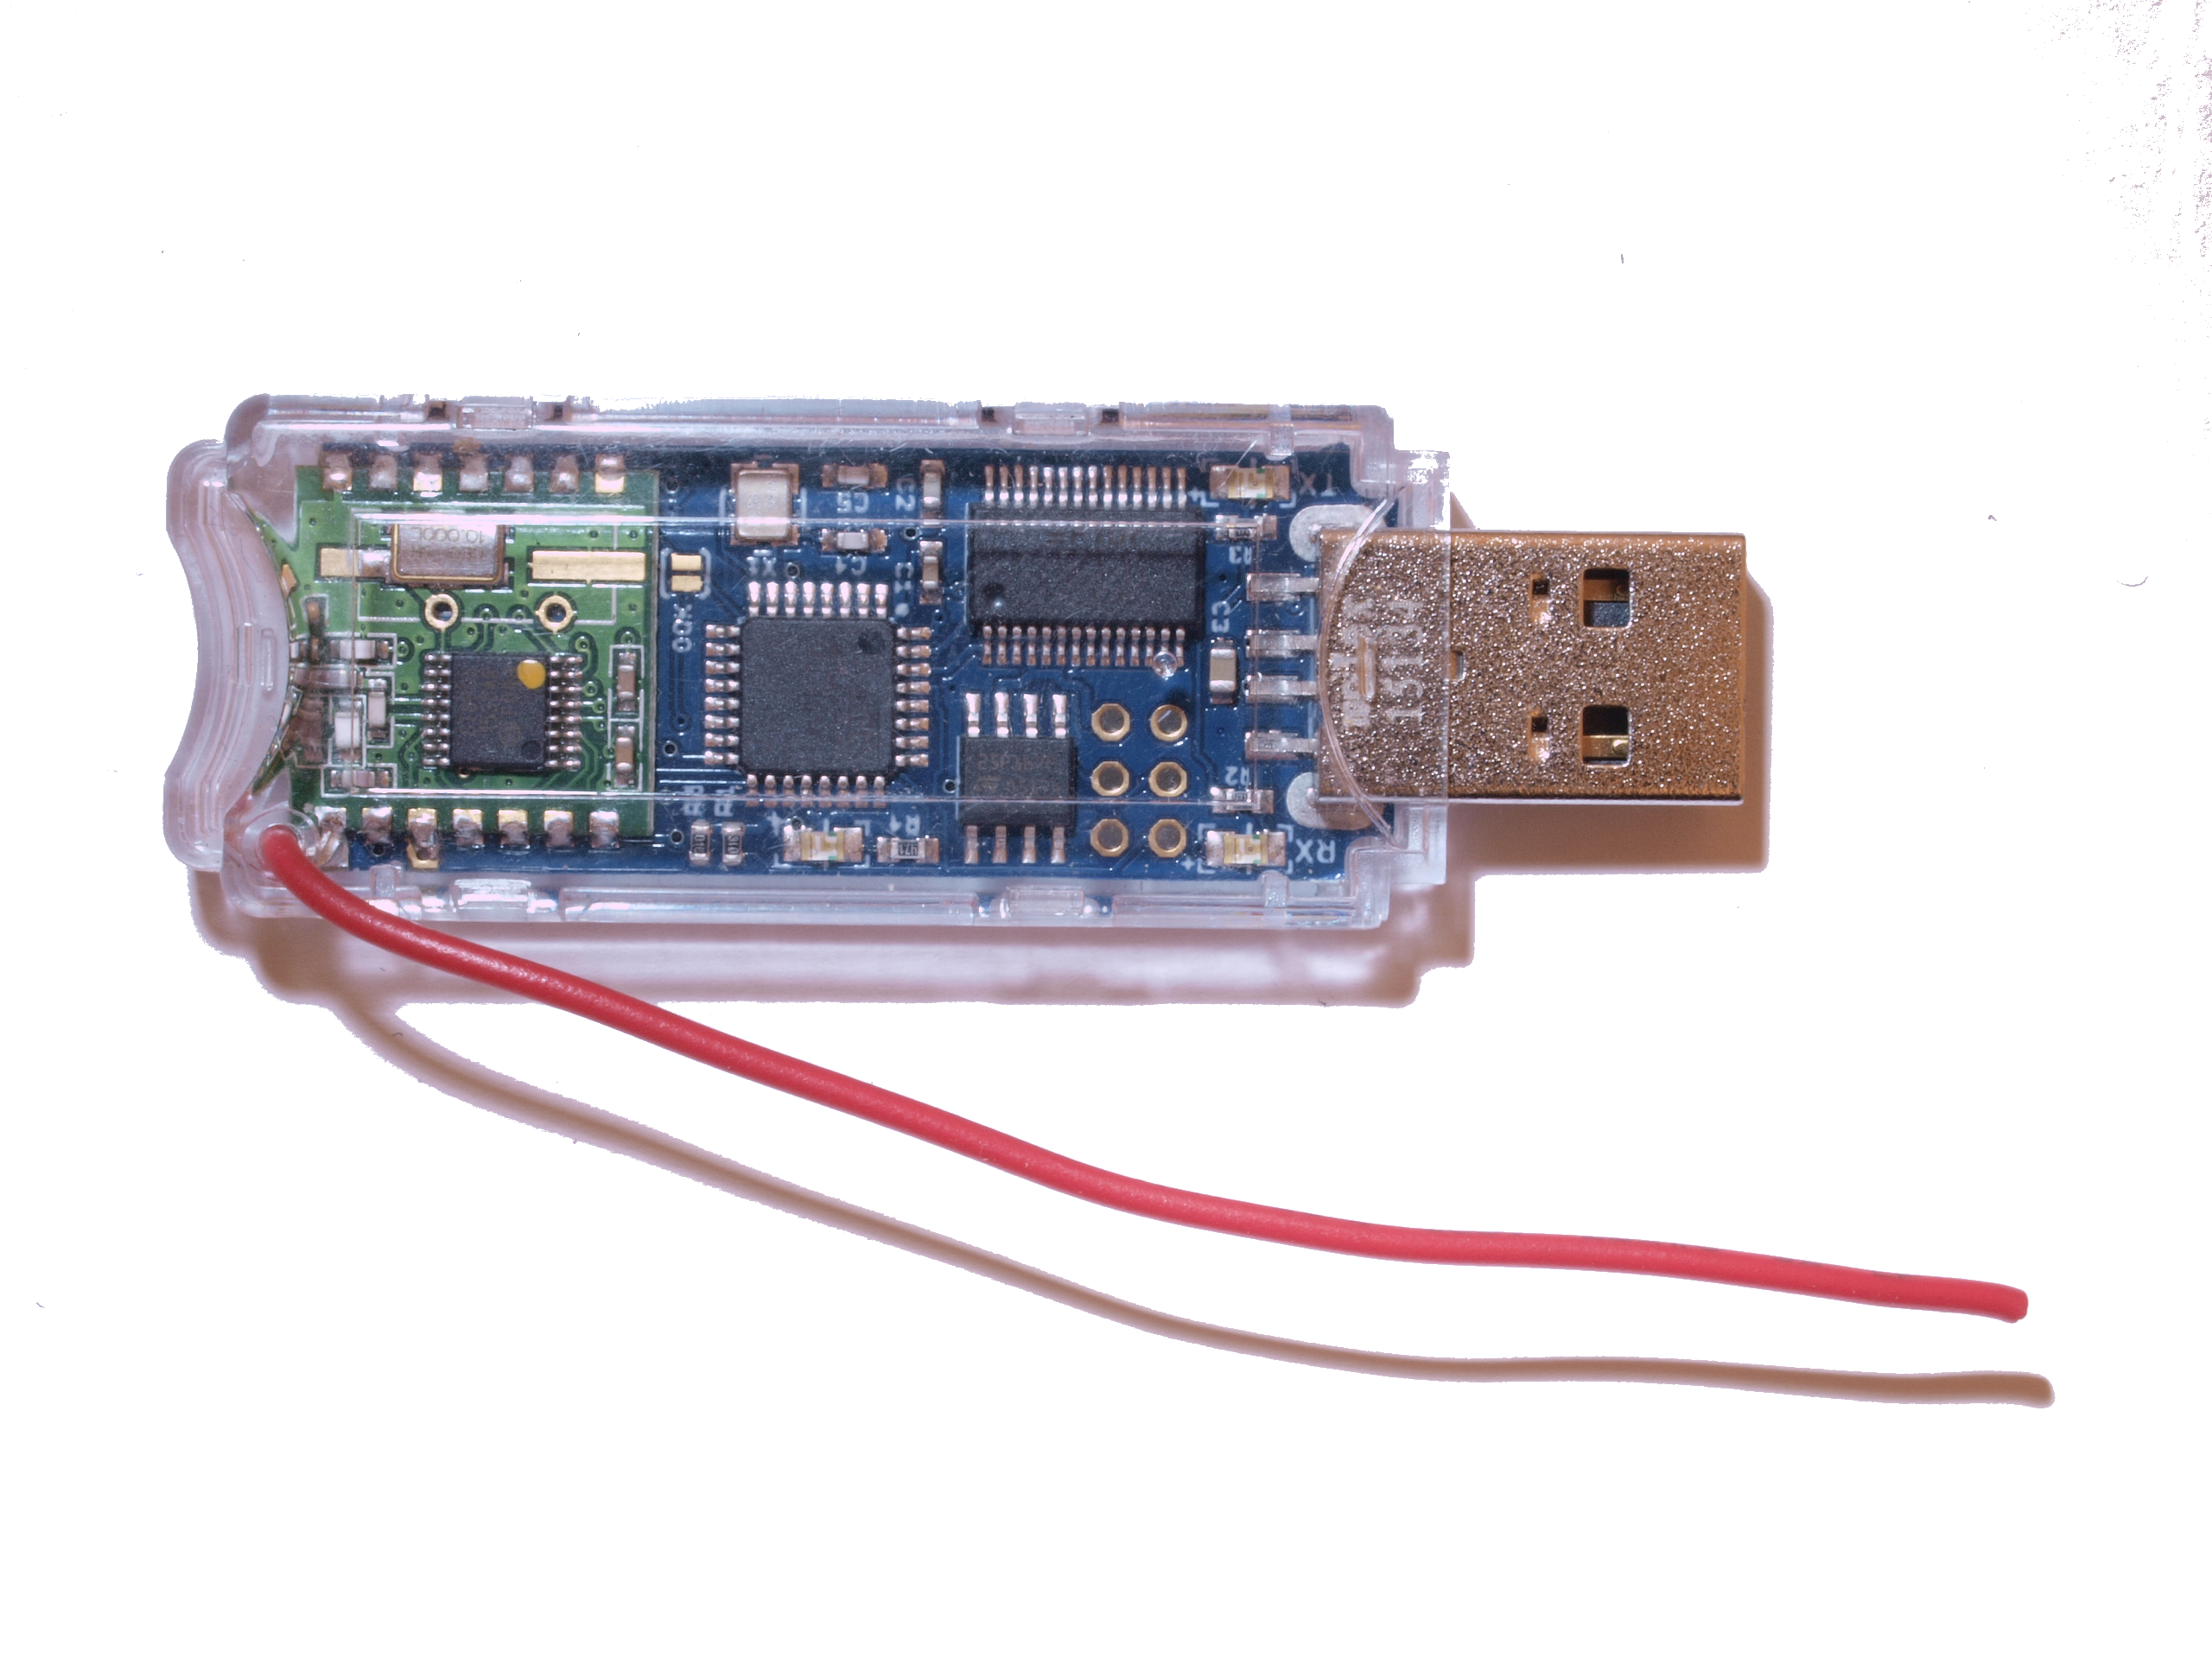
\includegraphics[width=0.48\textwidth]{../images/jeelink.png}
  \end{center}
  \caption{JeeLink}
  \label{fig:jeelink}
\end{wrapfigure}

\paragraph{JeeNode USB and JeeLink}\label{par:jeeLink}
Devices selected for the network are JeeLink nodes \cite{JeeLink} (figure \ref{fig:jeelink} shows the device). In addition to that, also several JeeNode devices \cite{JeeNode} (shown on figure \ref{fig:jeenode}) were obtained. These two devices are very similar in many ways and can interact with each other; JeeNode USB is only a little bit more versatile in its use options.



\begin{wrapfigure}{r}{0.5\textwidth}
  \vspace{-20pt}
  \begin{center}
    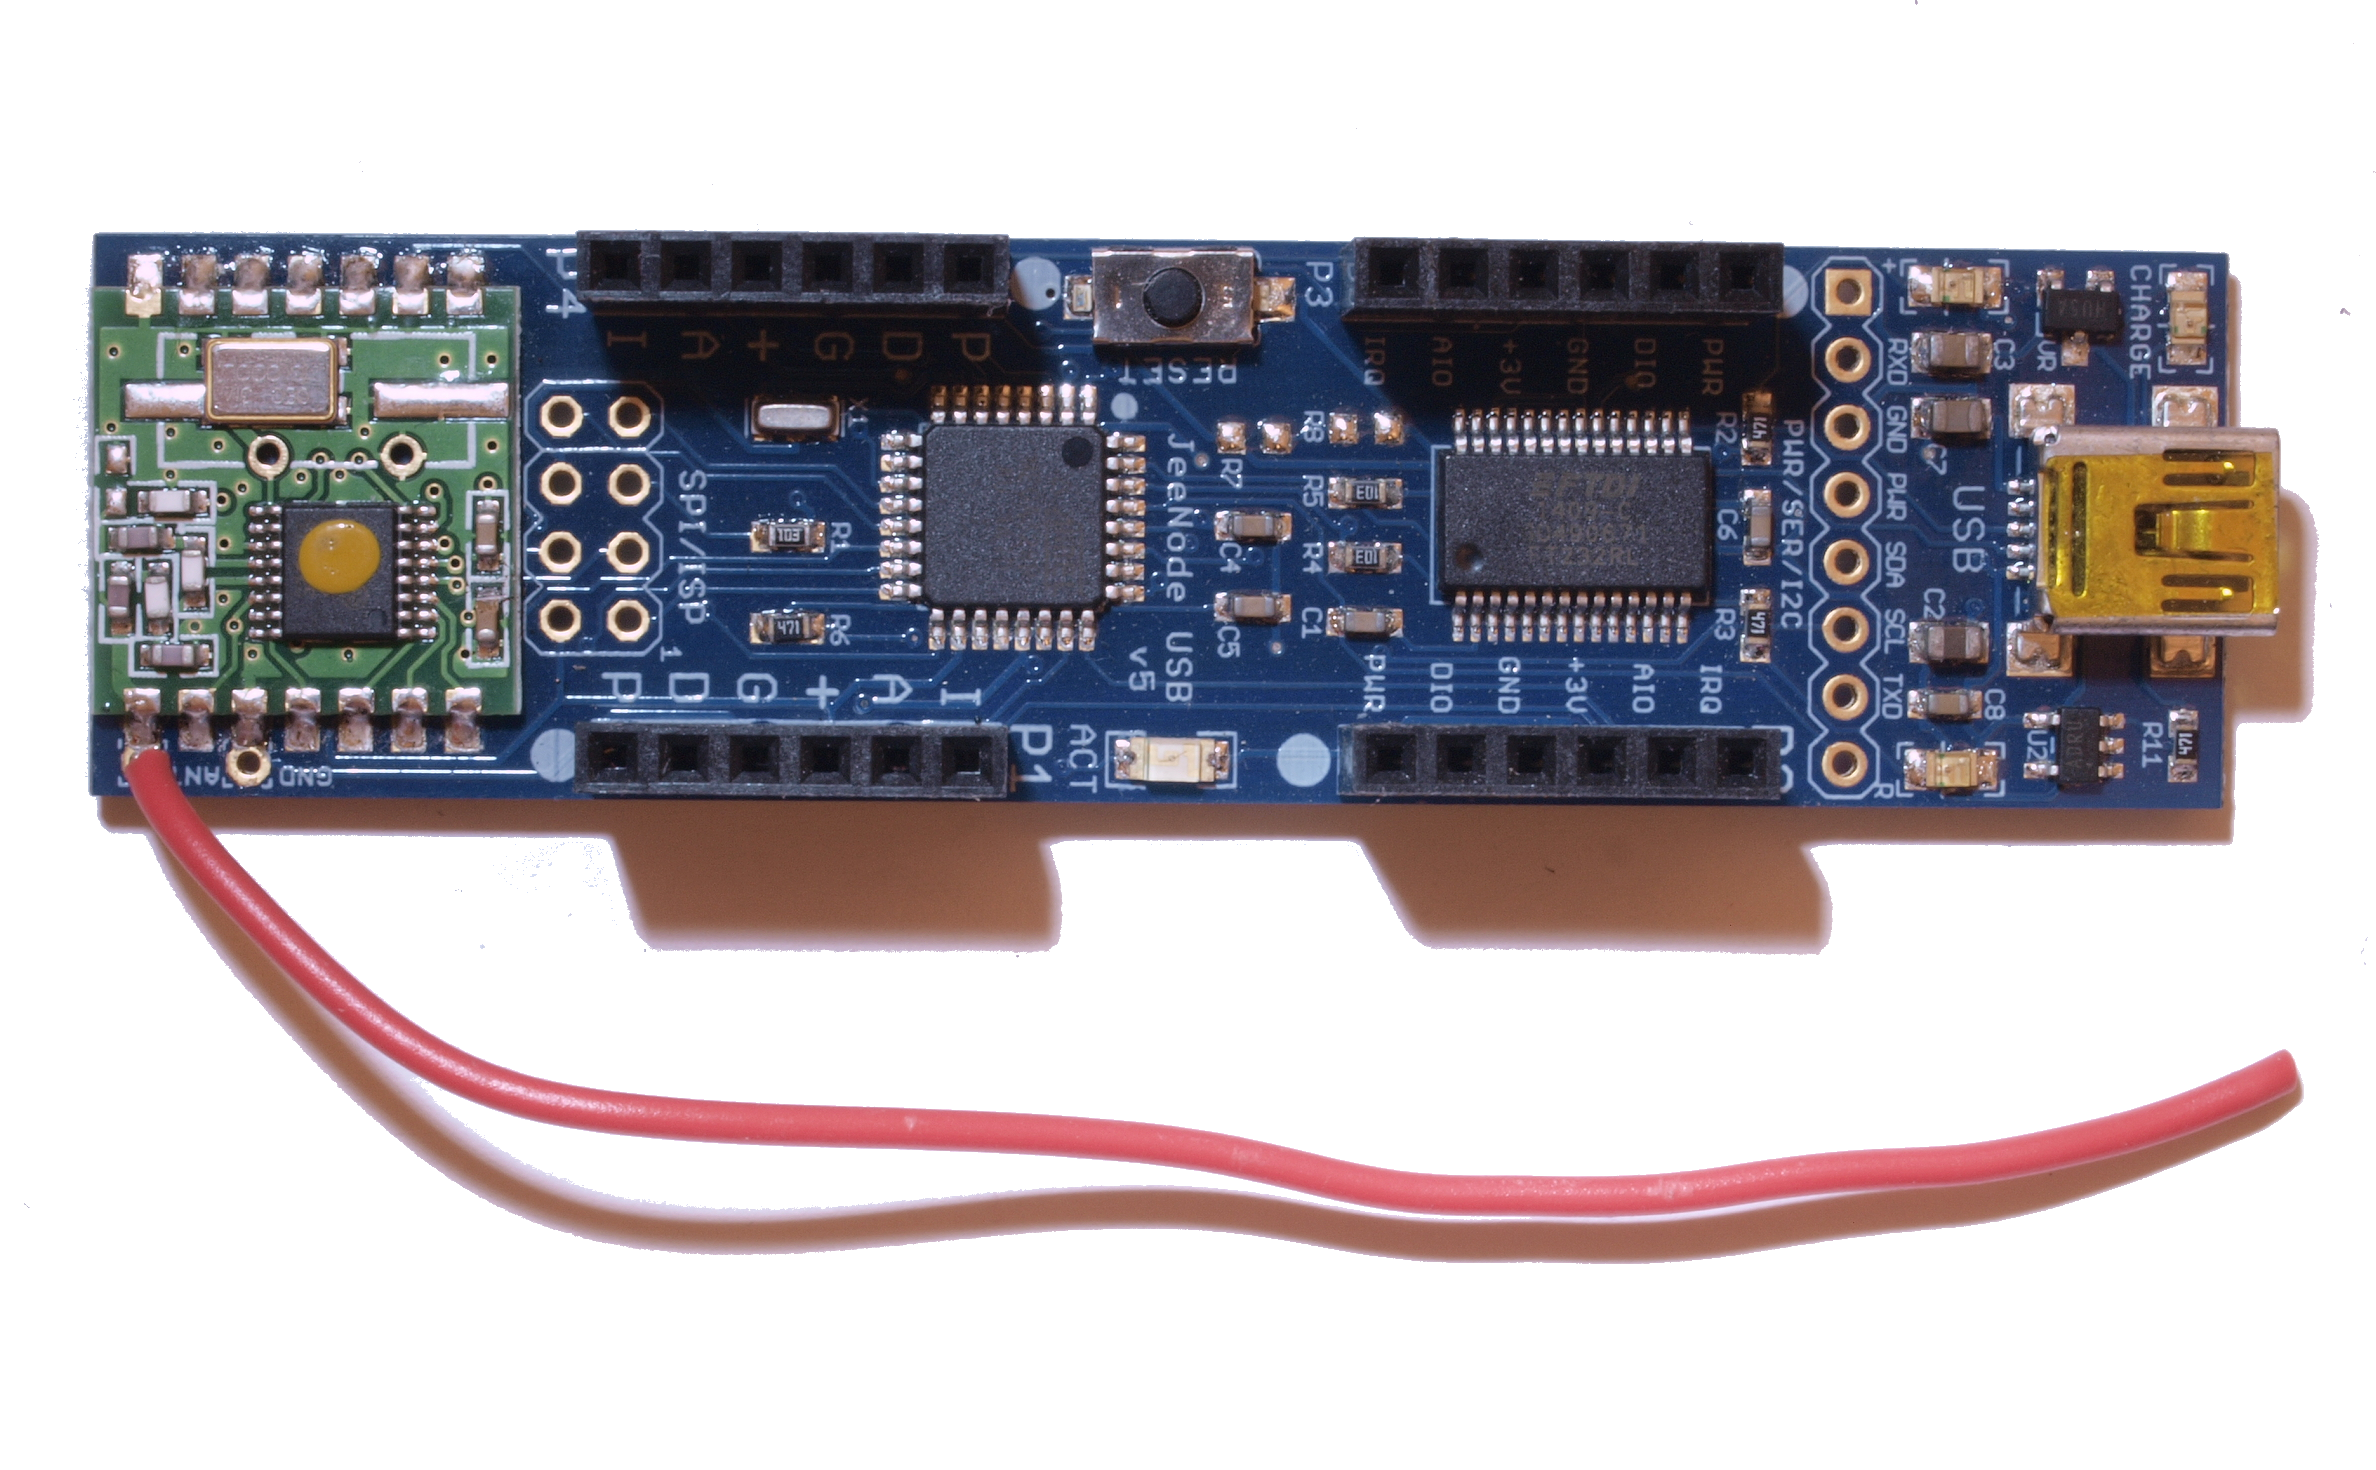
\includegraphics[width=0.48\textwidth]{../images/jeenode.png}
  \end{center}
  \caption{JeeNode USB}
  \label{fig:jeenode}
\end{wrapfigure}

Both of these devices are based on Arduino Mini \cite{ArduinoMini}
(version with ATmega328P processor). Wireless communication is enabled by the RF12B chip \cite{RF12B} (unmounted radio chip shown on figure \ref{fig:radio}) which is permanently mounted to the device. Both devices can be connected directly to a computer via USB\footnote{the USB port type one of the few differences}. The visual difference between these two devices is caused by the fact that JeeLink has a plastic cover. Therefore there is no additional connectivity. JeeNode is not covered, and there are pins available for additional sensors or any other devices. JeeLink has additional 16 Mbit of flash memory \cite{JeeLink} available. Therefore this can be used for convenient storage.

For both of these devices, there is accompanying library JeeLib \cite{JeeLib} that contains all necessary functions for controlling the radio. It also deals with any other features that are different from standard Arduino Mini.

\paragraph{RF12B radio module}\label{par:radio}
Simple and cheap radio module RF12B from HopeRF \cite{RF12B} is present on all JeeMote and JeeLink devices. The version sold in Europe is using 868 MHz frequency for the radio\footnote{other version can use 433 MHz or 915 MHz}. Like many other common radio modules, this radio is half-duplex. Therefore it is able either to receive or to transmit messages, but cannot do both at one time.

\begin{wrapfigure}{r}{0.5\textwidth}
  \vspace{-20pt}
  \begin{center}
    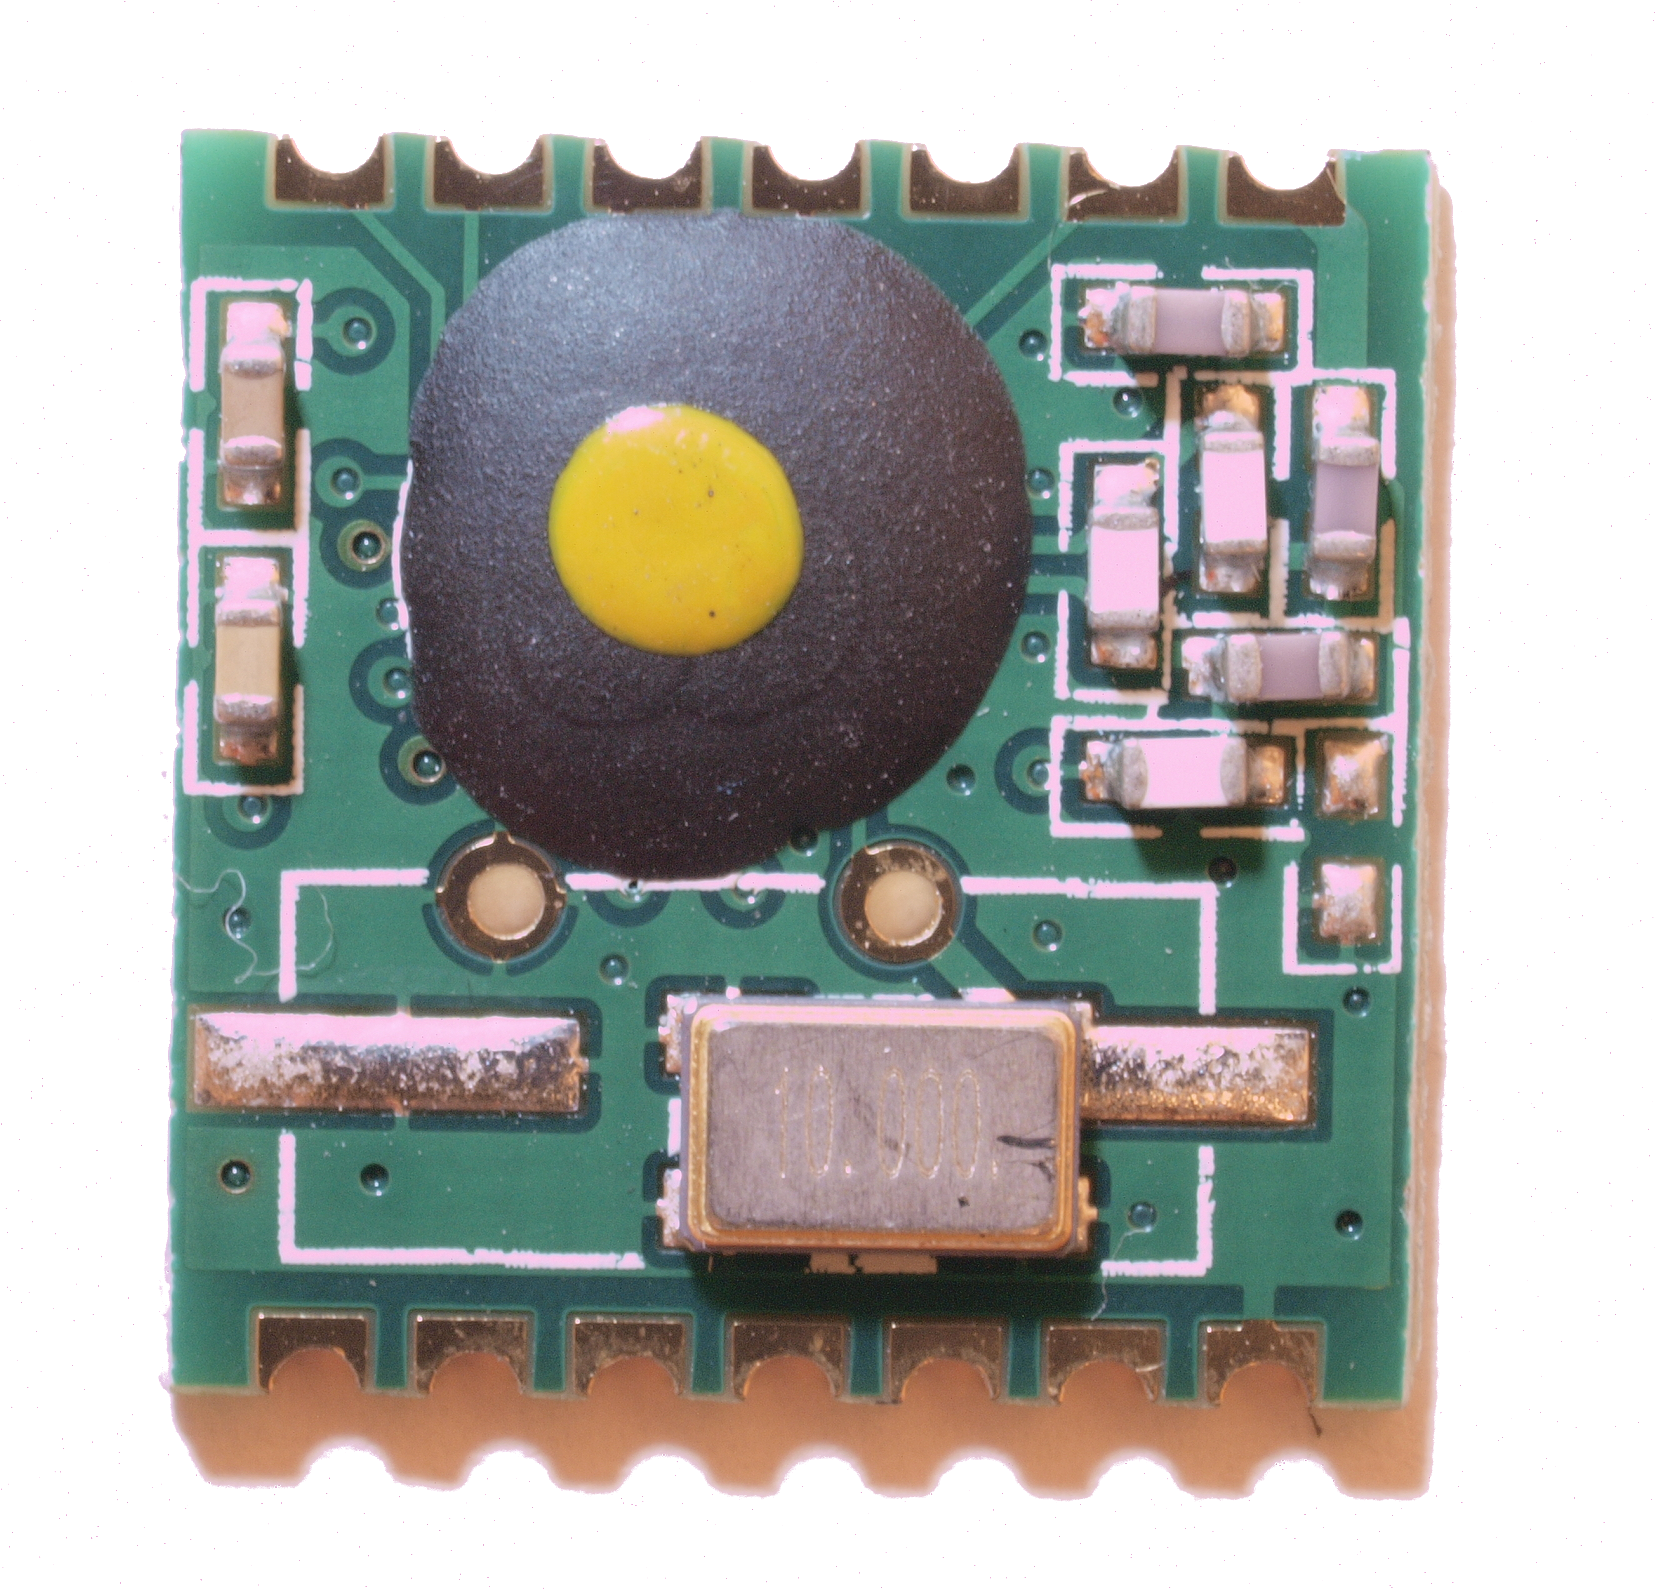
\includegraphics[width=0.2\textwidth]{../images/radio.png}
  \end{center}
  \caption{RF12B radio module}
  \label{fig:radio}
\end{wrapfigure}

The radio module is equipped with omnidirectional whip antenna ($\approx$ 8 cm long wire) by default. It is possible to modify the properties of such antenna by shaping it in various ways, e.g. straight wire compared to coiled one. There might also be many other versions and shapes of antennae, which might have an effect on radio properties, but this would be subject to whole another research in a different field.

\section{Node placement}\label{sec:place}
25 JeeLink nodes were deployed to achieve even coverage of the whole area. All devices are placed near the ceiling, where they are visible, but do not cause any obstructions. Due to a wire placement constraints, we decided to set these devices close to the walls. Plan with identified locations of each node can be seen in appendix \ref{fig:map} (each node is represented by a red triangle). The map shows only relative placement, exact coordinates together with IDs of each node can be found in the appendix in table \ref{tab:map}.

\section{JeeTool}\label{sec:jeetool}

%TODO short intro?

\paragraph{Motivation}
  Few nodes can be managed manually without any major problems, most frequently using  Arduino IDE \cite{Arduino} directly. This approach is working without problems for up to three devices, and it would be possible to manage more devices this way, but the usability is lowered with each addition.

  Either intentionally or not, there is no doubt that the official Arduino IDE is designed with simplicity in mind. Therefore it is usable for a person without a solid background in IT \cite{ArduinoIntro}. On the other hand, this simplicity comes at the cost of many features; that might have been useful for more advanced use (e.g. already mentioned management of multiple devices).

\paragraph{MoteTool inspiration}
  JeeTool \cite{JeeTool} was created to remedy this problem. A deployment tool that uses Arduino Makefile project \cite{ArduinoMK} to manage our testbed. This tool was inspired by motetool project \cite{motetool} which was developed by Dusan Klinec to manage the similar task, only for the different type of devices. The basic functionality is the same; it allows users to detect all connected devices and upload applications to the selected ones. Also, jeeTool includes support for bidirectional communication with individual devices via a serial port.

\paragraph{Implementation details}
  As has been stated, Arduino Makefile is used for the actual application upload. To make Makefile call for each of the connected devices, jeeTool creates temporary bash script file, which is used to set the environment for the specific node and execute the upload via Makefile. The temporary script itself is then executed with system call directly from jeeTool. If multiple nodes are selected for upload, jeeTool offers either serial deployment (mostly for debugging purposes) and parallel deployment, where all Makefile calls are made within discrete threads, thus all of them are executed simultaneously.

\paragraph{Communication over serial port}
  In addition to the upload features, jeeTool also enables communication with devices over a serial port. This is done via jSerialComm library \cite{jserial} at the moment. In the past RxTx library \cite{rxtx} was used, unfortunately, this library is currently not being developed\footnote{last update is from 2011}. Therefore we decided to change the library to more up to date one, instead of using problematic old code.

  Individual nodes are matched with files, which are named after the nodes (name of the device in the Linux file system). JeeTool is capable of writing all inbound communication in such file or read such file and write it over to the serial port. For the inbound communication, there is an option of delayed termination of the program. Thus jeeTool can be left running for specified amount of time before the ports to devices are closed (e.g. collect results after the experiment). For the outbound communication, jeeTool can send the whole content of the file at once, or there is an option of delay between individual lines of the file (can be used for periodic sending of messages, etc.).



%%%%%%%%%%%%%%%%%%%%%%%%%%%%%%%%%%%%%%%%%%%%%%%%%%%%%%%%%%%%%%%%%%%%%
\chapter{Research use}\label{ch:research}
  This chapter describes our case study for key generation mechanism without any pre-shared information between individual nodes.

  In today's application this would be quite a common problem since a number of devices equipped with some kind of radio module are constantly growing. Let it be Wi-Fi, Bluetooth, or any other frequency and specification. However, prolem for these devices is source of randomness. Many of these devices are too small or their price is too low, therefore they do not come with true random number generator. Thus key derivation is a bit challenge on these devices.

  Results of Mathur et.al. \cite{Mathur2008Rssi} show scheme for key derivation without any shared secret, only using properties of radio channel shared between these two devices and the nature of radio wave propagation through such shared channel. We show that this algorithm can be used in WSN environment.

  \section{Keys from radio signal}
  Due to a nature of a wireless channel which is not perfect, we can observe fluctuations and disturbances in the wave propagation. It might seem difficult at first to measure these since by no means we are able to observe all such events. Almost every radio module is able to measure RSSI\footnote{received signal strength indication}, which can be described as an amount of power in the received signal. There are many arbitrary scales and absolute values do not match on devices from different manufacturers since RSSI is relative index \cite{RSSIMeaning}.

  However, our algorithm can work regardless of the differences in devices. Even two devices with the same configuration can produce different absolute values due to antenna position and overall device manufacturing differences. (many of these devices are partially assembled by hand \footnote{e.g. JeeNode motes come as a ready to assemble kit}.)

  \subsection{Quantization principle}
    Quantization enables extraction of bits from individual values of signal strength. There are many different solutions to this problem \cite{Jana2009Rssi}, two main approaches here are: lossless quantization \cite{Azimi-Sadjadi2010Fading} and contrary to that we have lossy quantization \cite{Mathur2008Rssi}. %TODO quant. is inherently lossy

    Quantization is always lossy by design, we transform analog measurements of RSSI to single bits. However, the difference between two mentioned aproaches is number of generated bits per original RSSI measurements. Lossless quantization produces bit value from every measurement of signal strength, which is useful for high-performance demands, but it requires guaranteed variance in the radio channel (e.g. the nodes are constantly moving, or the environment is changing) Otherwise, the resulting keys could possibly be very weak.

    Lossy quantization, on the other hand, does not have guaranteed output length per number of measured values, which can lead to a very limited length of output sequences. However, this kind of quantization is expected to have better results in static environments \cite{Jana2009Rssi} because of its nature to drop such bits, that fail to differ from others.

    Since our network is static and without any moving nodes, we implemented lossy quantizer algorithm designed by Mathur et.al. \cite{Mathur2008Rssi}, which showed promising results for the off-the-shelf wireless devices. Authors also provided experimental results from scenarios comparable to our conditions.

    \subsection{Quantization algorithm}\label{subsec:quant}

    %general principle and image from suman jana
    \begin{figure}[h!!]
      \begin{center}
        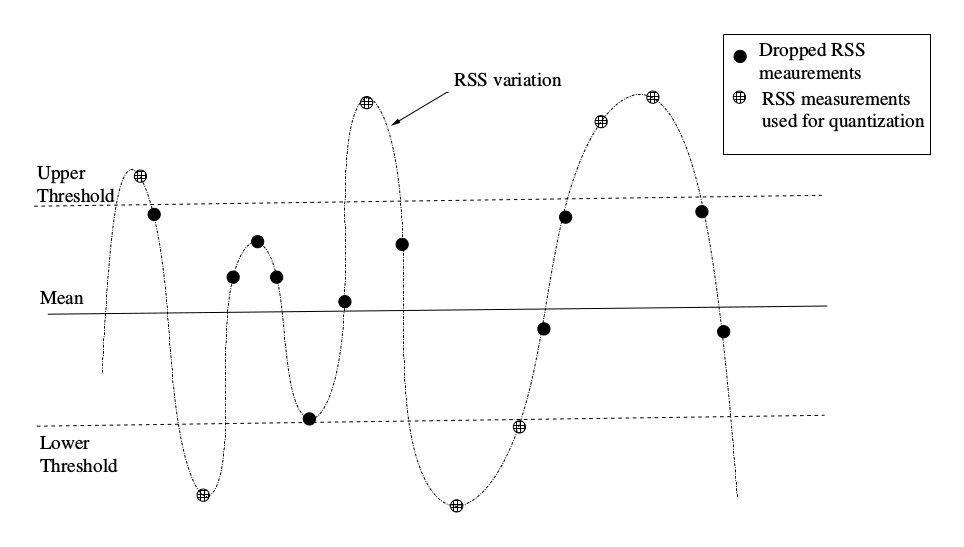
\includegraphics[width=\textwidth]{../images/quant_alg.png}
      \end{center}
      \caption{Sample quantizer. Values between tresholds are dropped. Values greater than the upper treshold are encoded as 1, values below lower treshold are encoded as 0. Therefore the output in this case will be 1010011 \cite{Jana2009Rssi}.}
      \label{fig:quant_alg}
    \end{figure}

    Nodes A and B exchange messages between each other, preferably at high rate of exchanged messages. Each node records RSSI measurement for every received message, thus both nodes record time series of RSSI values.     These values are processed and treshold is computed. It depend on the alghorithm whether one or multiple tresholds are used. Finally we process RSSI measurement once again, all measurements above treshold are treated as bit value 1 and all measurements below treshold as bit value 0. In case of multiple tresholds we drop measurements in between. Example with two tresholds is shown on figure \ref{fig:quant_alg}.

    Quantization princeple designed by Mathur et.al. \cite{Mathur2008Rssi}
     works as follows:

    \begin{enumerate}
      \item Both nodes send $n$ messages to each other in alternating pattern. Counter value is placed inside these messages, which is used to synchronise messages on nodes. For every one of these messages, signal strength is measured upon reception.
      \item When $n$ messages have been successfully exchanged, both nodes can proceed to the computational part.
      \item Both nodes calculate mean $m$ and standard deviation $sd$ for signal strength values of all received messages.
      \item Both nodes calculate $q^+$ and $q^-$ values, which are upper and lower quantizer bin boundaries, as follows:
      $$q^+ = m + \alpha \cdot sd$$
      $$q^- = m - \alpha \cdot sd$$
      \item Every signal strength measurement is then processed and it is rejected, if it lies within $q^+$ and $q^-$ boundaries, values above this range are assigned a bit value of one, values below are assigned a bit value of zero.
      \item Nodes then synchronise their measurement by exchanging list of counter values, where signal strength measurements were assigned either one or zero bit values.
      \item Counter values that match on both nodes are expected to be excursions in the same direction and are used to produce the resulting bit sequence.
      \item Final bit sequence can be also created in different way. Consecutive measurements on one side of treshold can be treated as one outcome instead of multiple ones.
    \end{enumerate}

  \section{Improvement strategies}
  As we can see from data collected in experiments during undisturbed network \ref{src:plain}, there no bits generated and that is the case for most of the time. To deal with this problem we have to introduce some form of artifical noise or disturbances.
  \subsection{Cooperative jamming}\label{subsec:jammer}
  The solution that offers itself is the help of other nodes within the network, because all of them are equiped with radio and we only have to work around the media access control mechanism in order to make two or more of them broadcast at the same time. Such idea has aready been researched, e.g. in work of Goel et.al. \cite{Goel2008Noise} or by He et.al. \cite{He2010Jamming}.



  \subsection{Other means of disturbances}\label{subsec:people}
  \subsubsection{People}\label{subsubsec:people}
  At first we tried to avoid this kind of disturbance as much as was possible, because movement of people is unpredictable (to certain extend) and such experiments are very hard (nearly impossible) to replicate.
  \subsubsection{Mechanical obstructions}\label{subsec:shield}
  TODO add shielding description with drawing

  \section{Experiment setting}
  An application was created, in order to collect data from a real-world network. Such data then would be processed by quantization algorithm \ref{subsec:quant} and produced bit sequences were analysed regarding the entropy and usability for cryptographic keys \ref{sec:results}.

  This application uses specially modified JeeNode motes \ref{sec:hw}, because analog RSSI values are not available through provided connections to radio module. Fortunately, analogue RSSI can be obtained through short jumper wire from radio module to the Arduino analog pin %CITE.

  In the experiment itself, two motes exchange messages with a counter value (counter is updated only on one of these motes) and both motes save measured RSSI values for each message. The counter value is used to guarantee delivery of these messages, mote A sends a message with value $n$ and mote B upon reception responds with the same value $n$. Mote A can increment counter value only when respond message with current counter value is received. Otherwise the same counter value $n$ has to be sent again and both motes will keep the RSSI measurement only from the most recent message with counter $n$.

  The application is programmed in such way, that 1000 counter values are exchanged, then they are sending out via the serial port and application is terminated. Intervals between individual messages should be as short as possible so that the random disturbances in the radio channel would be captured on both nodes. Even though RSSI measurement is definitely not symmetrical, using this approach we can expect them to be highly correlated %CITE.

  The limit of 1000 messages was set due to the memory constraints of individual devices. Since the bottleneck of our experiment was in the communication via the serial port, we opted to exchange all messages and gather data first and only after that to transfer them out to the server. The application was then uploaded to the nodes again and run from fresh state several times as the experiment settings required. In the optimal conditions, the expected time for a single run of application is about 30 seconds; runtime over two minutes is usually a result of some kind of error, either in the application itself, placement of devices, or disturbances in the radio channel.

\subsection{Attacker model}

  In addition to regular nodes, up to two sniffer motes were active at the time of application runtime. These were uploaded with modified version of an application, so that they would only receive messages, but would not send any messages to other devices. We have done several trials on a placement of these sniffer motes, in order to see any impact of position in the network on the results.
TODO


  %TODO plan of mote placement


  \section{Performance Evaluation (results from experiments)}\label{sec:results}
  We have made several runs of our application with different settings. Nodes A and B were always on the same places (sniffer positions were altered), but the conditions of radio channel itself were different. First, as a base level, we had run the experiment in conditions without any disturbances. After we realised, that the plain static network does not produce any usable data, we tried to introduce other techniques \ref{subsec:jammer} \ref{subsec:people} that would add disturbances to the radio channel, therefore changes in the measured RSSI values.

  To analyse the gathered data we used set of R scripts %CITE R
  and all data postprocessing was done outside of the motes, while in the real settings, motes would have to do all of the computations on their own. In orde to evaluate produced bit sequences, we used min-entropy \ref{par:min} and frequency test \ref{par:freq}, both on eight and four-bit chunks of data. The goal was to obtain several measurements of entropy in the data and then use the most conservative of them to estimate contained randomness. Since we had collected only small amounts of data for individual sources, we decided not to use any of statistical test batteries %CITE
  , because our data either did not match the required amount of input or the results would not be statistically significant for such small sample.

  \paragraph{Min entropy}\label{par:min}
Min-entropy \cite{barker2012recommendation} is considered the most conservative estimate of unpredictability in information theory. To make a min-entropy estimate of IID\footnote{Independend and identically distributed} source we can use simple calculation as follows, given the dataset with N samples:


\begin{enumerate}
  \item Find the most frequent value and let $C_{MAX}$ equal number of occurences of this value in dataset.
  \item $pmax = \frac{C_{MAX}}{N}$
  \item $C_{BOUND}=C_{MAX} + 2.3 \cdot \sqrt{N \cdot pmax \cdot ( 1- pmax)}$
  \item $H = - \log_2 (\frac{C_{BOUND}}{N}) $
  \item $W$ is the number of bits in each sample of dataset.
  \item Min entropy is then equal to $\min(W, H)$

\end{enumerate}

It is important to note, that this calculation of min-entropy estimate is only meaningful for IID sources \cite{barker2012recommendation}, for non-IID sources we have to use other means. Testing sources with dependencies with this min-entropy calculation may result in overestimates and generally output without any meaningful use.

There are many tests for estimating min-entropy contained within the output of non-IID sources, most notably collision test, partial collection test or the compression test \cite{barker2012recommendation}. To us the most meaningful one was the frequency test\cite{barker2012recommendation}, because of its ability to work on small amounts of data, a larger amount of data only increase the accuracy, but the test can provide a meaningful estimate on any amount of data provided.

\paragraph{Frequency test}\label{par:freq}
  On first sight, the calculation is similar to the original min-entropy \ref{par:min}. The calculation is following, using $0.005$ as confidence level $\alpha$:

  \begin{enumerate}
    \item Count occurences of each value in the dataset as $count_i$ for all $i=1 \dots n$ where $n$ means all possible outputs.
    \item Calculate $\epsilon$ from confidence level $\alpha$ and number of observations in dataset.
    $$\epsilon = \sqrt{\frac{\log(\frac{1}{1-\alpha})}{2\cdot N}}$$
    \item $pmax$ is the probability of most likely observation value.
    $$pmax = max_{i=1..n}(\frac{count_i}{N})$$
    \item Resulting estimate of min entropy is
    $$min-entropy =  -\log_2 (pmax + \epsilon)$$

  \end{enumerate}

  Using these two approaches we can get the most conservative estimate of entropy contained within our gathered data.

  Results from all experiments are summarised in the table \ref{tab:sources} and then results for each individual source are discussed in following subsections.

  \begin{table}[h!!!]
    \begin{tabularx}{\textwidth}{llllX}
      \hline
      Sources: & Plain & Jammer & \begin{tabular}{@{}l@{}}  Moving \\ people\end{tabular} & \begin{tabular}{@{}l@{}}  Moving \\ shielding\end{tabular} \\
      \hline

      Total runs: & 40 & 10 & 424 & 26 \\
      \begin{tabular}{@{}l@{}}  Usable runs I.\\ ($sd \neq 0$)\end{tabular}&  0 & 0 & 256 & 25 \\
      \begin{tabular}{@{}l@{}}  Avg. bits \\ produced I.\end{tabular}&  0 & 0 & 189.41 & 238.48 \\
\hline
      \begin{tabular}{@{}l@{}}  Avg. errors \\ produced\end{tabular}&  - & - & 0.41 & 0.00 \\
      \begin{tabular}{@{}l@{}}  Avg. errors \\ on sniffer\end{tabular}&  - & - & 51.00 & 59.88 \\
\hline
      \begin{tabular}{@{}l@{}}  Usable runs II.\\ (Both 1s and 0s in output) \end{tabular}&  - & - & 97 & 10 \\
      \begin{tabular}{@{}l@{}}  Avg. bits \\ produced II.\end{tabular}&  - & - & 409.06 & 470.00 \\
\hline
      \begin{tabular}{@{}l@{}}  Min entropy\\ (8bit chunks)\end{tabular}&  - & - & 25.96 & 34.21 \\
      \begin{tabular}{@{}l@{}}  Min entropy\\ (4bit chunks)\end{tabular}&  - & - & 50.64 & 68.39 \\
      \begin{tabular}{@{}l@{}}  Frequency test\\ (8bit chunks)\end{tabular}&  - & - & 42.45 & 52.62 \\
      \begin{tabular}{@{}l@{}}  Frequency test\\ (4bit chunks)\end{tabular}&  - & - & 72.40 & 96.01 \\

      \hline

    \end{tabularx}
    \caption{table of sources evaluation}
    \label{tab:sources}
  \end{table}
  \subsection{Plain source}\label{src:plain}
  As we can see from the table \ref{tab:sources}, there were no bits produced from this experiment. The reason behind is really simple, there were no disturbances in the %FORCE
  radio channel, therefore all measurements of RSSI resulted in the same value. Therefore the quantization algorithm \ref{subsec:quant} computes $sd$ equal to 0, thus fails to establish bounds $q^+$ and $q^-$ and there are no bits produced on the output. Sample visualisation can be seen in figure \ref{fig:rssi_01}.

  Since there are no bits produced, there is no point in measuring the entropy of the output. This result can be considered as the pitfall of static networks, without any moving parts or changes in the environment, there is not enough entropy in the radio channel as such, that could be used to extract entropy because there is none. Of course, the greater the area such network covers, disturbances are more probable, but we have to be aware of this problem and be prepared to identify such environment. The main reason being any bits generated in such environment should not be used \cite{Jana2009Rssi}.

  \subsection{Jammer}\label{src:jammer}
  Friendly jamming can be used as a possible remedy to the problem of static network \ref{subsec:jammer}, creating artificial noise in the network and thus possibly adding some entropy (given that the jamming is not predictable).

  As the results in the table \ref{tab:sources} show, this approach was not successful, mostly because of limitations of used radio modules \ref{par:radio}. While this approach would work with more advanced radios that are capable of subtractions on the signal level and allow for more devices to broadcast at one time. RF12 radio module and its accompanying library, however, does not allow this, mostly because of really simple collision avoidance algorithm. The approach is based on simple principle, not to send messages when there is any other signal present in the wireless medium.

  Therefore our primitive jammer, although jammer itself was able to broadcast anytime, failed. The legitimate nodes A and B could not receive nor broadcast their own messages, because of the collision avoidance. Thus the only effect of jammer was prolonged time needed to exchange 1000 messages between devices.

  To counter this behaviour, we tried to limit the transmission power used by sniffer, even using it without antenna. Once the signal was limited to the required level, that nodes A and B would not be interrupted by it, then we observed same results as if the jammer was not present at all.

  Although there might be other option how to make this approach work, because we limited ourselves to using stock radio modules and available software for radio management, we were not able to produce any bits using this method.
  Thus we leave out this option for either more advanced users (who might be able to control the radio on the most elemental level, therefore defining own collision avoidance rules etc.) or users with more specialised hardware (e.g. software defined radio modules). %CITE

  \subsection{Moving people}\label{src:people}
  This option was not one of the originally intended sources, but during the experiment with plain source, we discovered, that people walking through the monitored area caused much-wanted irregularities in a radio signal. This option would be a viable for busy places like already tried cafeteria \cite{Mathur2008Rssi} or town square. Thanks to the network placement we utilised our classroom and made these measurements during one of the lectures. The data clearly show some patterns, mostly we can observe timeframes which produce bit sequences with high entropy and also timeframes where no bits were generated.

  \begin{figure}
    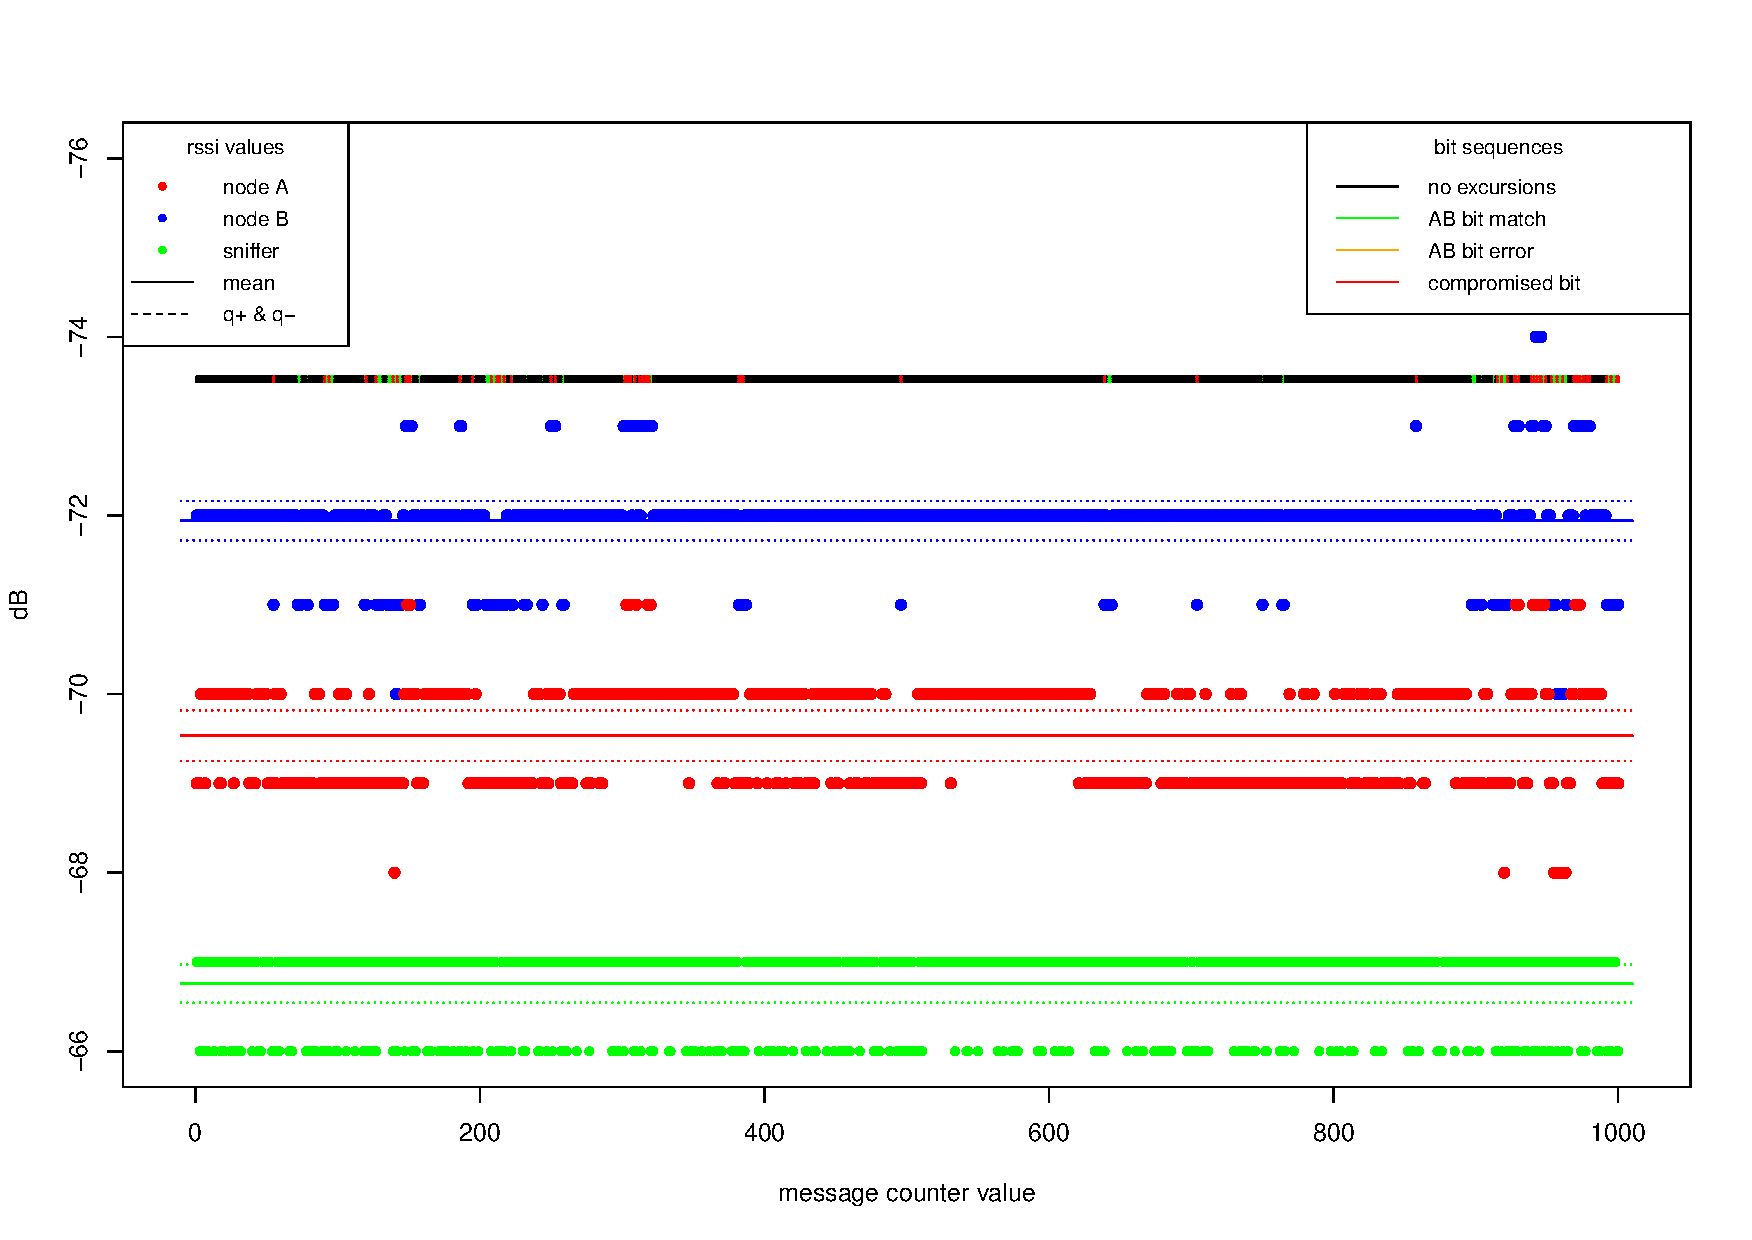
\includegraphics[height=\textwidth, angle = 90]{../images/graph_rssi_04.pdf}
  \caption{TODO add numbers to description}
  \label{fig:rssi_04}
  \end{figure}


  These differences can by explained by a simple fact, people do not move in a random fashion. And that is exactly what we can observe in our data, during runs, that produced data people were moving, but most of the time they remained stationary, therefore with almost no effect on the network. Although movement of people is not random, it is can be considered not predictable, therefore it might be sufficient source of randomness for our purposes.


  One sample run from this experiment is shown as figure \ref{fig:rssi_04}. From this run, there were 161 bits generated, with zero errors between nodes A and B. And sniffer node made 90 errors, thus about half of the bit sequence was compromised.

  The results show promising values and show us, that there is a potential and more research should be done in this direction. We can see a clear trend in data, once we filter out unusable runs (either because no bits were produced, or because produced bit sequence contained only zeroes), we can see, that about one-quarter of runs is suitable for bit extraction. Of course, these runs are not evenly distributed in our sample, they are rather clustered. On average, we can generate about 400 bits from one successful run. As we can see from the results of min-entropy \ref{par:min} and frequency test \ref{par:freq}, the most conservative estimate is about 26 bits of entropy contained within these data. Thus on average we would like to utilise five consecutive runs, in order to generate a usable key.

  \subsection{Moving shielding}\label{src:shield}
  In the last experiment, motivated by the promising data from previous one, we tried to introduce disturbances in the radio channel without the presence of any person \ref{subsec:shield}. In the table we can see, that this approach achieved almost the same results as the previous one \ref{src:people}.

  Unfortunately, due to an error, we did not manage to collect any larger amount of data, therefore there is not much we can conclude from these results. However, the current results are promising, averages of generated bits and entropy estimates are slightly better than in other experiments.  These values might decrease with more experiments, but given the fact, that these results were produced on a network without any interference from outside, this area is definitely worth looking into.

  The big question regarding this source is the predictability of such data, because as we can see on graph of sample run \ref{fig:rssi_02}
  there are clearly visible excursions that do repeat in somewhat regular fashion.


  \subsection{Speed (bits of key per time)}
  One run (exchange of 1000 messages) takes approximately 30 seconds to complete. This is under a condition, that these two nodes are only one to use the wireless medium, otherwise the required time would be different.

  Anyway, approximately 30 seconds to exchange values and then some minor time for calculations and exchange of two messages with identified excursions (which are negligible regarding the time).  From these 1000 values we can obtain about 25 bits of entropy on average \ref{src:people}, therefore we can gather about 50 bits per minute.

  This is comparable to the original result 1 bit/sec of Mathur et.al. \cite{Mathur2008Rssi}, however, we were capable of exchanging way fewer messages per minute than the original proposal (our rate 1000 msgs/30 sec is not comparable to 4000 msgs/sec achieved by Mathur et.al.), probably due to the nature of used devices \ref{sec:hw}.
  \subsection{Possible errors}
  Question about reliability surely comes to mind. We have no direct guarantee, values and measurement on individual nodes are clearly not symmetrical, we only expect them to be highly correlated.

  As we can see on the boxplots \ref{fig:errorsT} \ref{fig:errorsS}, the errors between nodes A and B are indeed scarce, therefore there is reasonable probability, that the nodes A and B will be able to establish the common key, using the obtained bit sequence from quantization algorithm \ref{subsec:quant}.

  The other important part is how many bits were compromised to the sniffer node and potential attacker. As we can see, on average there is an hamming distance of 50 bits between output bit sequence for nodes A and B and bit sequence derived at sniffer node. Of course, there are excursions in both directions, therefore we cannot entirely guarantee that the derived bit sequence is secret.


  \begin{figure}
    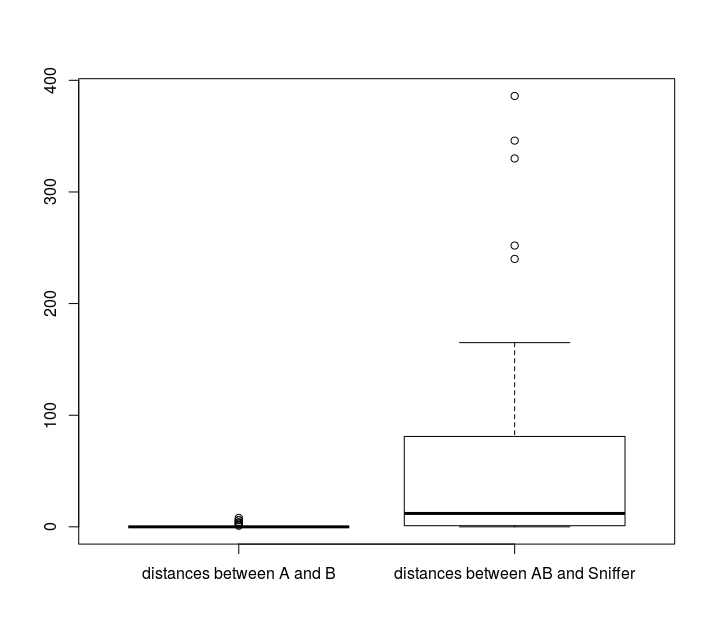
\includegraphics[width=\textwidth]{../images/boxplotDistancesTeaching.png}
  \caption{Boxplot of Hamming distances between generated bit sequences from nodes A, B, and sniffer node during movement of people \ref{src:people}}
  \label{fig:errorsT}
  \end{figure}

On the other hand, our bit sequence still needs some post processing in order to extract the randomness \ref{sec:use}, the most simple one would be a hash function. Therefore, if we use a correct function, we can expect, that one different bit would cause a change in half of the bits in the resulting key thanks to the avalanche effect \cite{Webster1986}.

We can clearly see, that guessing is also not an option, although individual bit positions in a sequence are known, there is no way to estimate whether the identified excursion is over or below the threshold. Guessing which bits are not correct is also not an option while guessing just one-bit change would mean $400$ trials on average, two bits would mean about $400^2$ trials. Complexity for this case grows exponentially and the sniffer gets $50$ bits wrong on average without any reasonable clue which bits are correct and which are not.

  \begin{figure}
    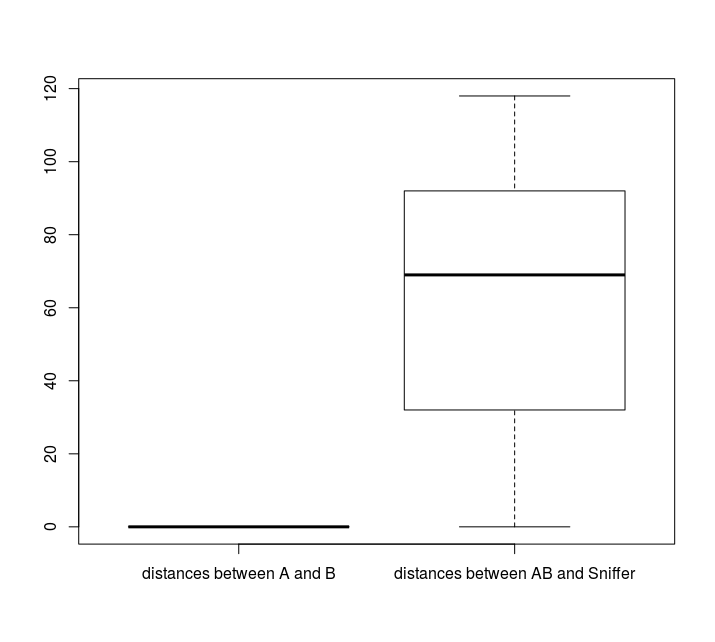
\includegraphics[width=\textwidth]{../images/boxplotDistancesRottation.png}
  \caption{Boxplot of Hamming distances between generated bit sequences from nodes A, B, and sniffer node during movement of shielding \ref{src:shield}}
  \label{fig:errorsS}
  \end{figure}

  \section{Discussion and use cases}\label{sec:use}


%%%%%%%%%%%%%%%%%%%%%%%%%%%%%%%%%%%%%%%%%%%%%%%%%%%%%%%%%%%%%%%%%%%%%
\chapter{Education use}\label{ch:edu}

  \section{motivation for educational WSN network}
  The current state of the art WSN devices usually uses specialised hardware and software in order to achieve the best performance available. %\CITE
  This, unfortunately, is not the ideal prerequisite for an easy to learn matter. In fact, most of WSN devices have rather complicated setup and are quite challenging for novices \cite{hu2010wireless}.

  Because of such discouragement, it is difficult to teach how to
  work with WSN’s; few hours (at least) are usually required
  to explain the basics, which is reasonable for a research project or
  something similar, but for a class exercise, this would turn out to be
  not the most effective use of time, if it would be achievable at all. And
  we have not yet mentioned more advanced topics in this area, such as
  common techniques for encryption or message authentication.

  Issue of this nature can be solved in various ways,
  in the case of Edu-hoc, we decided to sacrifice performance \ref{sec:hw}; which is not that much important for a network with an educational purpose. On the other hand, using hardware that is really easy to comprehend and use is of a great benefit here. Also having less powerful, but relatively cheap devices (in the range of \$30 rather than \$100 or more) gives the opportunity to lend each the students one of the devices, so that they can try the basics on their own, and also use this device for interactions with the network.

  \section{Scenario approach (attack and repair)}
  In order to make learning more enjoyable experience and also to add some challenging part to the learning process, we decided to make Edu-hoc scenario based; each scenario being composed of two distinct parts: first part in the role of an attacker (both enjoyable and educational) and the second part as a code reviewer or developer (primarily educational).

  \paragraph{attacker part of a scenario}\label{par:att}
    Students are presented with network application which has known, or easily detectable, vulnerability. Task is to take advantage of such vulnerability and exploit it using own nodes and carefully executed interactions with the network. How successful these efforts were can be easily evaluated by percentage difference from the expected traffic of the network or by presenting learned secret in the submission of the solution. Exact methods of evaluation are described in \ref{sec:eval}.

  \paragraph{reviewer part of a scenario}
    An important part of the educational process is not only to find mistakes, but also to be able to correct them. The task in this part of the scenario is then to take the current source code of an application, which has been deployed on the network during the attacker part \ref{par:att}, correctly identify which mistakes were made and propose changes in the code, which would make the application secure against such kind of an attack. Exact evaluation methods are again described in \ref{sec:eval}.


    \subsection{1st scenario - Eavesdropping}\label{subsec:1st}
    The first scenario can be considered really simple and it is by design. Since this scenario is the first encounter with Edu-hoc, we opted for passive attacker approach, without any actual interaction with the network, just listening for any traffic.

    Eavesdropping is also the first thing one would do if one would be about to attack some network because it does not compromise the presence of an attacker and intercepted messages may provide many useful pieces of information. This is another important reason why this task was selected as a first one, not only it is rather easy to do, but it provides vital information for the rest of the exercises (e.g. which nodes are present in the network, which frequency is used and what are the settings of the radio)

    \paragraph{scenario setting}
    Each node in the network sends messages, after each message, there is a delay of 1000 ms, therefore any receiving node has time to process the transmitted messages. All messages are sent as a broadcast and nodes within the network do not receive nor process them since it is not needed for successful scenario run. If this would be the case, transmission rates would have been updated accordingly and the scenario would be much more likely to fail on its own, because of single node malfunction, while with current settings, the network can operate without any problems even is several of the nodes would fail.

    \paragraph{attack principle}
    The attack is very simple, attacker node only has to listen for any traffic present in the network. For best results application has to be able to process as many messages as possible, however any performance changes will affect the end result only slightly (final percentage will be better, but the bottleneck is in the processor of the radio module, so better optimised application will increase the end result only by approximately 10-20\%)
    \paragraph{application and securing it}
    The main issue with the application is unencrypted broadcast. This can be fixed quite easily, just by the addition of simple encryption and for simplicity using common shared key. We have to be aware of the fact, that attacker might be able to collect some of the nodes and thus learn such key and compromise it and there are techniques which deal with this problem %CITE
    However, in our scenario, this is sufficient solution because it is adequate to measure against eavesdropping.

    \subsection{2nd scenario - Black hole attack} \label{subsec:2nd}
    This scenario presents more advanced concepts, dynamic routing in particular. The task is to attack the routing algorithm and diverse all traffic so that the central node does not receive any messages. This scenario requires active attacker, thus some basic interaction with the network.

    \paragraph{scenario setting}
    The scenario is divided into two parts, first parts are shorter and are used to establish routes for this particular run of scenario. Without any attack or interference outside from the network, these routes should be always the same.

    In the following part of scenario each node periodically sends messages to the parent node, therefore all messages are routed to the central node. This node then counts all received messages and the final outcome is the number of expected messages compared to the number of actual messages received.

    \paragraph{attack principle}
    This attack requires some prior knowledge before execution which can be obtained simply by using eavesdropping technique from the previous exercise. This way an attacker can learn how the routing algorithm works (nodes broadcast their current distance to the central node, where central node has distance of 0, all nodes that hear distance announcement message then update their distance and broadcast this updated distance)

    With this knowledge attacker than try to inject message with the same content as the central node does, but earlier than the central node is scheduled to do so. After this, the message from a central node will not improve the position of other nodes and they will not update their distance. Another possible approach is to find an intentional weakness in the algorithm implementation (application allows negative distance values).

    The only thing that remains is to make sure to use nonexisting ID within the network and after the routing tree is established, attacker node can simply disappear, because it is no longer needed.

    \paragraph{application and securing it}
    In order to fix the application one has to fix two issues; check for negative counter values (which is the easy part and requires usually addition of one condition within the code); and what is more important, implement some kind of authentication mechanism for messages from the central node, or otherwise make sure that the attacker cannot diverse all the traffic only by being a bit faster than the central node.

    Many options are available, the easiest one being preshared random authentication tag, which would be added to the messages. This is really simple countermeasure, but it guarantees that the attacker can't send a valid message before the central node sends it.

    \subsection{3rd scenario - Sinkhole attack}\label{subsec:3rd}
    Although very similar to the second scenario, this poses far greater challenge than the previous one. The goal is not only to divert the traffic but also modify it on the fly and send it to the original recipient.

    The greatest issue here is related to the performance, since all messages from the entire network will be routed through single attacker node, therefore most of the messages are very likely to be dropped somewhere in the process, because single node is not capable of receiving and processing messages from every other node in the network, if they do not transmit on very slow rate.

    Task for this scenario is to deliver a modified message to the central node before the original message is delivered; messages with the same identifier but different content are discarded and only the one which was received the earliest is kept at the central node.

    The reason why two very similar scenarios exist, while it could have been only this one, is to present scenarios in a manner of slowly increasing difficulty. If we were to skip the second scenario \ref{subsec:2nd}, the task might be too complicated to some, while this way, required task in the third scenario \ref{subsec:3rd} is only a minor extension to the second one, however, the achieved result is a far greater impact.

    \paragraph{scenario setting}
    Runtime of this scenario is the same as for the previous one \ref{subsec:2nd}; initial phase of route establishment and after that messages are routed from nodes to the central node. The expected outcome is to divert ad modify as many messages as possible.

    \paragraph{attack principle}
    The first part of the attack can be executed in the same fashion as the previous one \ref{subsec:2nd} although it is not the ideal way. As the goal is not to prevent all messages from reaching its destination, but to deliver as many modified messages as possible. Therefore it is not a good idea to modify all of the routes in the network, but only as much as the attacker node is capable of handling (i.e. only third of the nodes in the network). This can be done by sending the distance message only to selected nodes instead of broadcasting it.

    Another part of the attack is rather simple, attacker node has to receive all messages which are addressed to it, modify these messages as it is required and send these messages to the central node. Modification usually requires simple text substitution inside the body of the message or task very similar to this one.

    \paragraph{application and securing it}
    Again as many times with this scenario, the fix is partly the same as per second scenario \ref{subsec:2nd}, which deals with the attack on the routing; either preventing it or detecting it.

    The another part of this fix is primarily an authentication problem, therefore any kind of MAC will be able to secure this application. Therefore the problem of shared key arises again, but as before in first scenario \ref{subsec:1st} one master key will be able to do the job, if we assume, that the attacker does not have access to individual devices, only to radio communication between them.

    The point of the exercise is to deal the problem at hand without complicating it with anything else. Of course, we could add any advanced key distribution schemes  %CITE
    to the application in order to add countermeasures against master key compromise, but that would make completely different application without any real added value to the original educational purpose.

    \subsection{4th scenario - Jamming} \label{subsec:4th}
    Evey once a while attacker comes around a network, application or protocol which is designed with security in mind, meaning there are no backdoors or weak spots in the design or implementation (really idealistic scenario, however, it is very likely that the attacker does not resource to find or use existing vulnerabilities, thus for such attacker there is no real way how to exploit such application).

    Nevertheless, it is very likely that such attacker would like to cause any kind of damage he is capable of doing. Most likely to make the application, protocol, or network unavailable; most likely by DoS attack %CITE
    or something similar. For wireless communication it is quite easy to do, since the wireless medium, air to be specific, can be used by only one device at a time. If an attacker is able to utilise all ate available slot for transmissions, then the legitimate user would not be able to transmit anything. Such technique is called jamming and it is quite easy to deploy.

    \paragraph{scenario setting}
    The setting of this scenario is really simple, all nodes send a message via the fixed routing tree to the central node, who the counts the number of delivered messages. There is no phase of route establishment, only the message delivery phase. The assignment is to prevent delivery of as many messages as possible. Since there is no option to modify the routes etc. the only reasonable way is jamming.

    \paragraph{attack principle}
    As has been stated before, jamming is the expected way of solving this scenario, although there might be many creative solutions created. With jamming one can either bypass the media access protocol and send data continually, thus preventing everyone else from sending any messages, or the another viable option is to send many valid messages to the central node, thus overloading it and forcing this node to drop many incoming messages, including the valid ones.

    \paragraph{application and securing it}
    Since this attack does not exploit any weakness, only the actual property of wireless communication and network design, there is not much one can do to prevent such attack, while only modifying the application source code. However, there are ways of dealing with such kind of an attack. Countermeasures are usually based on multiplication of the devices and decentralisation of the whole network. Therefore give two or even more nodes the ability to become the central node, use multiple frequencies etc. %CITE

  \section{Evaluation principle}\label{sec:eval}
  Measuring the success can be done in various different ways, Edu-hoc utilises few different methods to decide, whether the attack was successful and how big was the impact of an attack.

  Evaluation for each scenario is a little bit different because there are different objectives. The task of first scenario \ref{subsec:1st} is to capture as many messages as possible, therefore the evaluation is done as a simple comparison between the set of captured messages and set of pre-computed messages that are known to be transmitted in the time period of scenario run. Comparing these two inputs line by line we get intersect of these two sets, that contains all successfully captured messages and is stripped of all the duplicates and possible fraud messages. A number of messages in the resulting is then compared to the expected number of messages in order to receive the final percentage evaluation, the higher the number, the better the result.

  The second and the fourth scenario \ref{subsec:2nd} \ref{subsec:4th} have the same goal, only differ in the scenario settings, which can be omitted for the evaluation purposes. The common goal is to prevent as many messages as possible from delivery to the central node. The way it is done is rather simple, the central node counts every delivered message and the resulting number is compared with the expected amount of messages.

  Unfortunately, this design of scenario lacks in the evaluation one important thing, the credit for the attack cannot be given to any participant, because we have no identifier involved. Messages only vanish, but we do not know, whether it was by joint work of multiple attackers, one really successful one or by a fault in the network itself. Therefore there is not much of use for such scenario in the courses, and because of this, modified versions of scenarios have been used \ref{sec:PA197}.

  The third scenario \ref{subsec:3rd} however utilises message modification, which can be used for identification purposes. Therefore messages on the central node are not only counted, but alco compared to the expected ones and differences are noted\footnote{the amount of computation on this level would limit the usability of the node, thus the node only sends received messages over the serial port to the server, where the actual evaluation is done}.

  Since students are assigned a unique identifier to modify the messages with, we can easily distinguish between participants and evaluate how successful they were in this task.

  The last option which can be utilised in evaluation is a submission of secret, which was received from interaction with the network, node either responds to received message with such secret or the secret has to be extracted from the communication in the network. Such secret can be a short word, number or something of similar nature and again such secret can be unique for each participant, which makes te evaluation an easy task.
  \section{Web interface and auto run}
  Edu-hoc was designed as a long-term exercise, thus single scenarios are expected to run for days, possibly week or longer. However, for some, it would be extremely impractical to repeat only once during the whole time because we would like to present fresh scenario to everyone involved,  and also we would like to reset the scenario once a while. This will ensure correct initial settings and if we set the intervals right, then everyone will be able to test out several solutions within a reasonably short timeframe.

  To achieve such kind of behaviour, we can utilise various approaches, the easiest one being set of bash scripts and setting the cron service %CITE
  accordingly. The other option might be modified JeeTool, which would be running continuously and in set intervals would trigger the corresponding action.

  The last option is the most complicated one but offers the most

  \section{PA197 use and results} \label{sec:PA197}

%%%%%%%%%%%%%%%%%%%%%%%%%%%%%%%%%%%%%%%%%%%%%%%%%%%%%%%%%%%%%%%%%%%%%
\chapter{Future and related work}\
  \section{RSSI}
  \section{Edu-hoc}
\chapter{Summary}




%%bibliography
%%==============================================================
{\csname captions\languagename\endcsname %% Temporarily override
%% the BibLaTeX localization with the original babel definitions.
\makeatletter %% Use the correct localization of the quotations.
  \thesis@selectLocale{\thesis@locale}\makeatother
\printbibliography[heading=bibintoc]} %% Print the bibliography.
%%==============================================================

\appendix %% Start the appendices.
\chapter{Testbed map and node placement}
\begin{figure}[h!!!]
  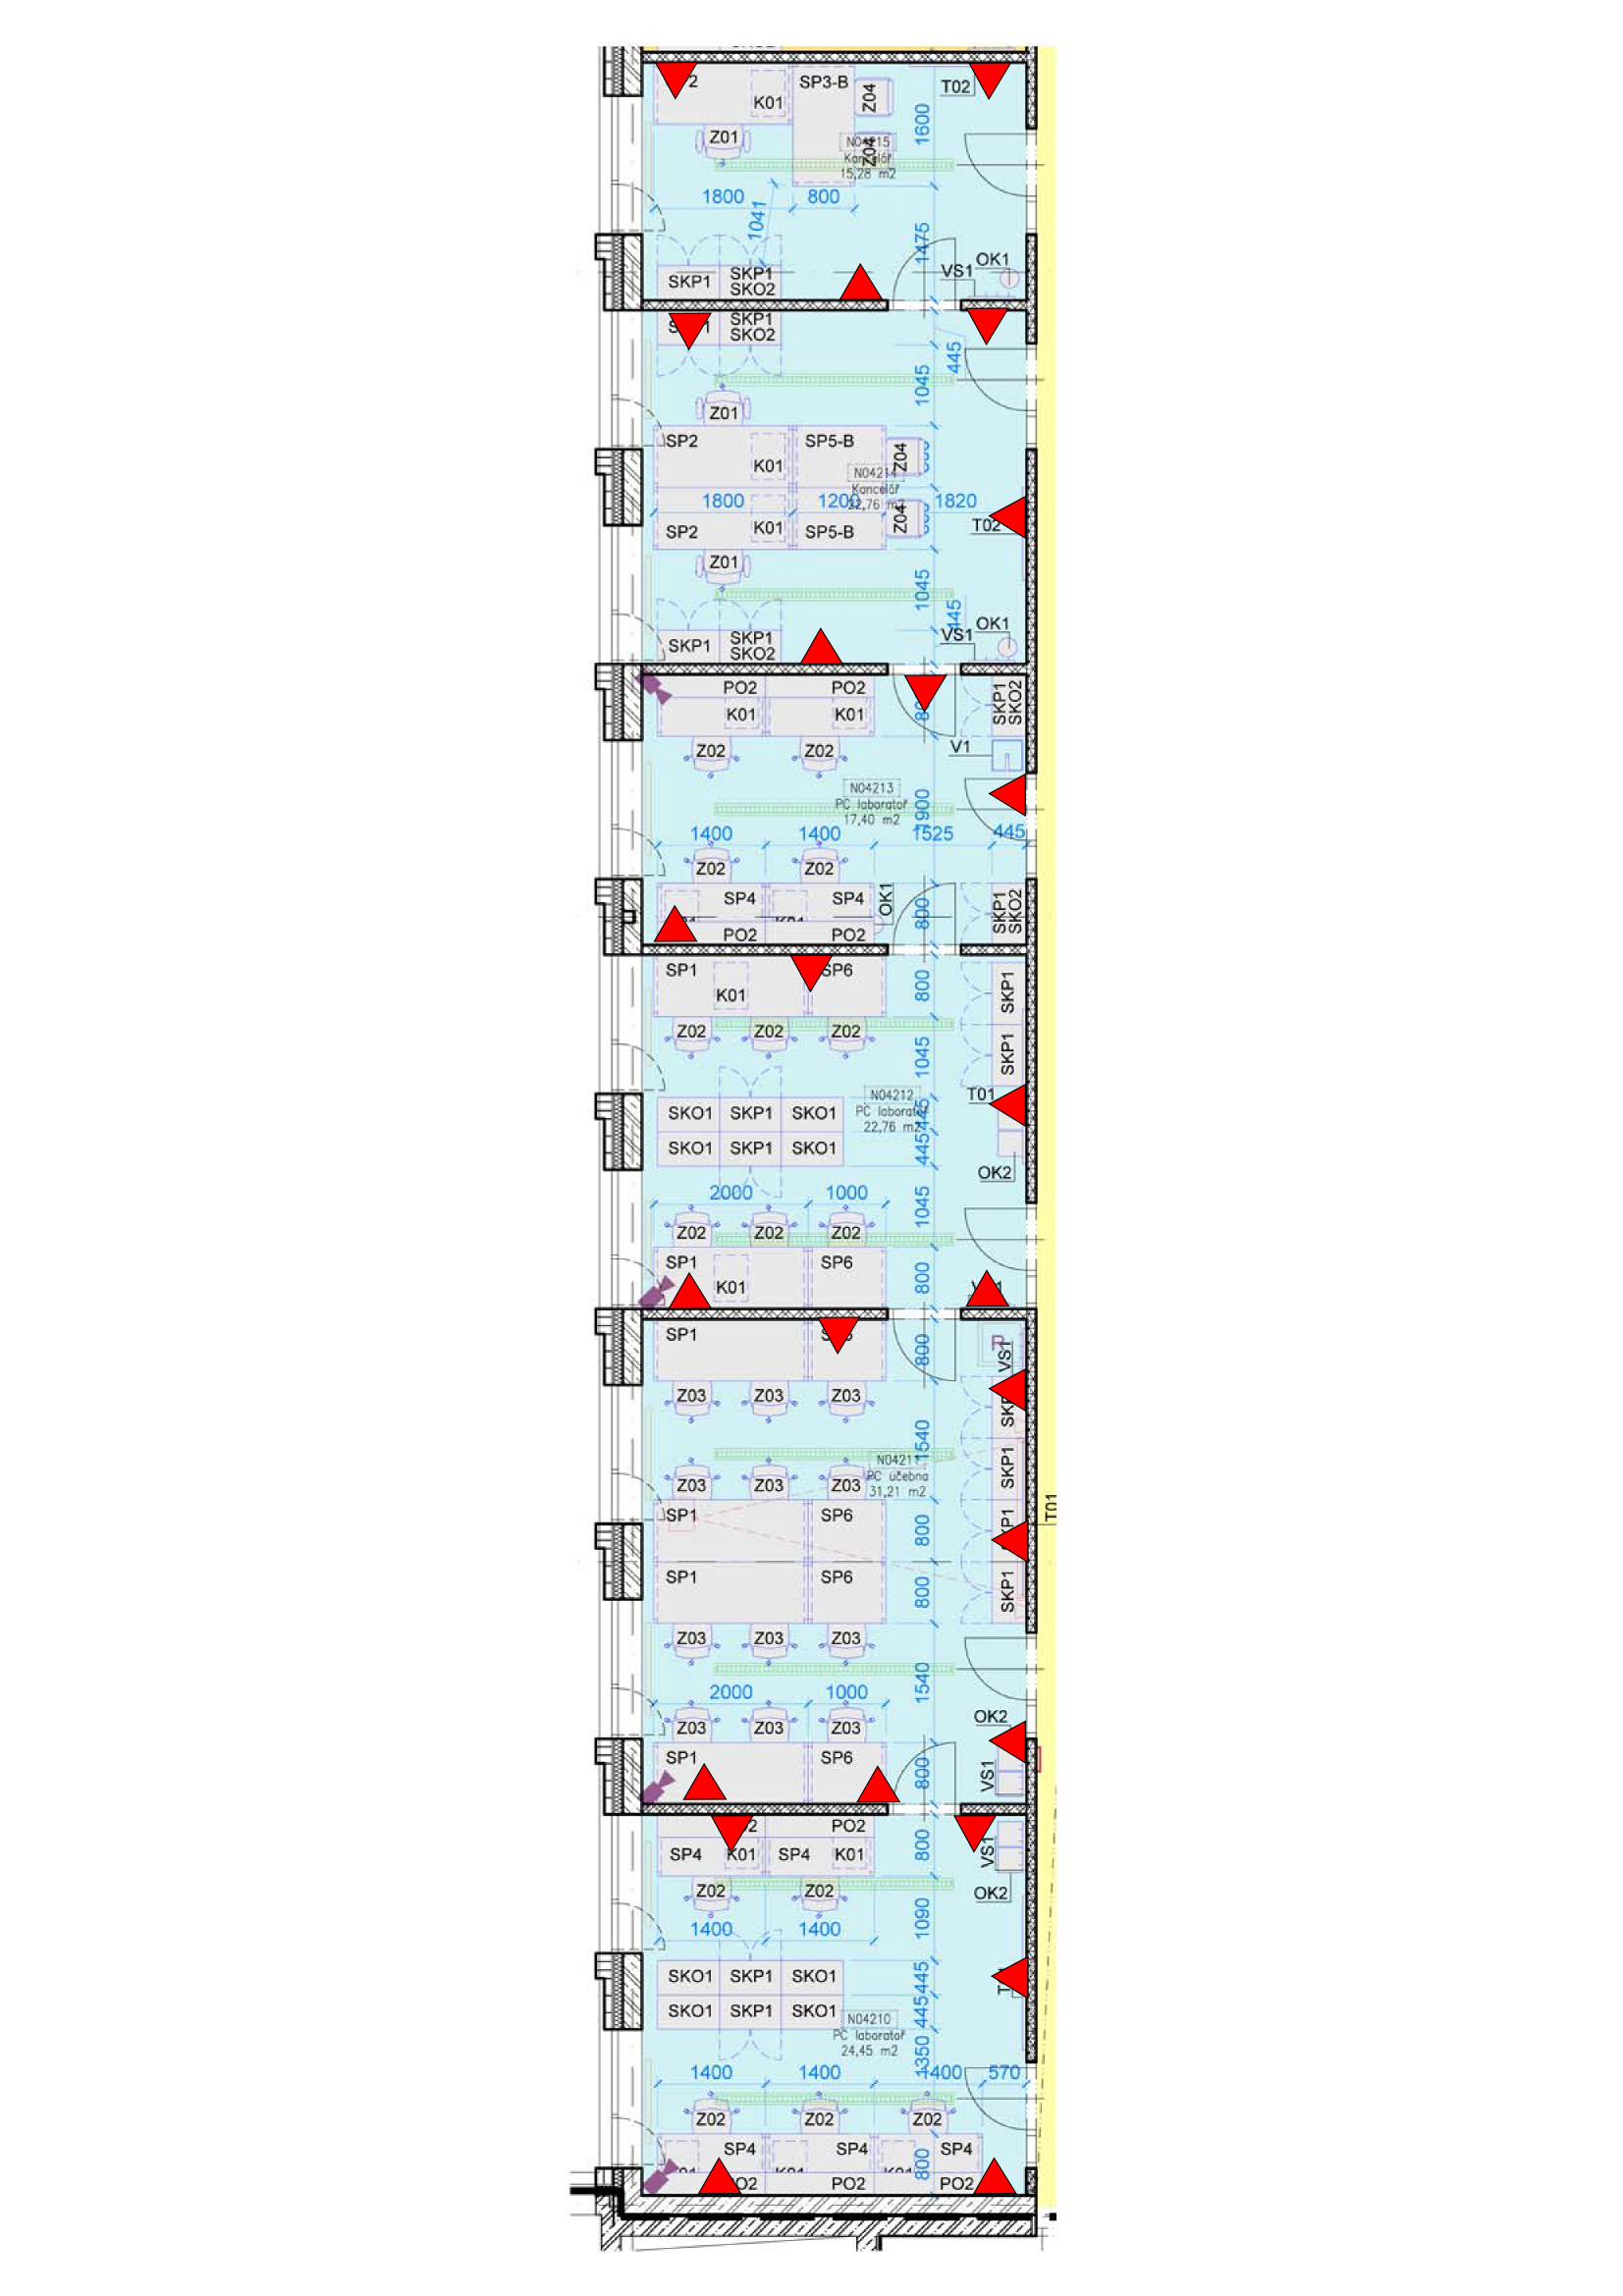
\includegraphics[width=0.9\textwidth]{../images/testbed.png}
\caption{Map of testbed with placement of individual nodes}
\label{fig:map}
\end{figure}

\begin{table}[h!!!]
  \begin{tabularx}{120px}{c|cc}

id &    x &    y\\
\midrule
1 &    1498 &    0\\
2 &    1977 &    207\\
3 &    1147 &    90\\
4 &    1147 &    447\\
5 &    1134 &    0\\
6 &    1134 &    310\\
7 &    949 &    0\\
8 &    506 &    65\\
9 &    506 &    475\\
10 &    1718 &    0\\
11 &    1964 &    242\\
12 &    1616 &    462\\
13 &    1603 &    490\\
14 &    2434 &    0\\
15 &    2434 &    500\\
16 &    2214 &    0\\
17 &    2447 &    295\\
18 &    2753 &    70\\
19 &    2753 &    320\\
20 &    333 &    0\\
21 &    493 &    390\\
22 &    493 &    70\\
23 &    155 &    0\\
24 &    0 &    210\\


\end{tabularx}
\caption[Node IDs and placement coordinates]{Node IDs and placement coordinates\protect\footnotemark}

\label{tab:map}
\end{table}
\footnotetext{Coordinates begin from top right corner of map}


\newpage
\chapter{RSSI graphs}
\begin{figure}[h!!!]
  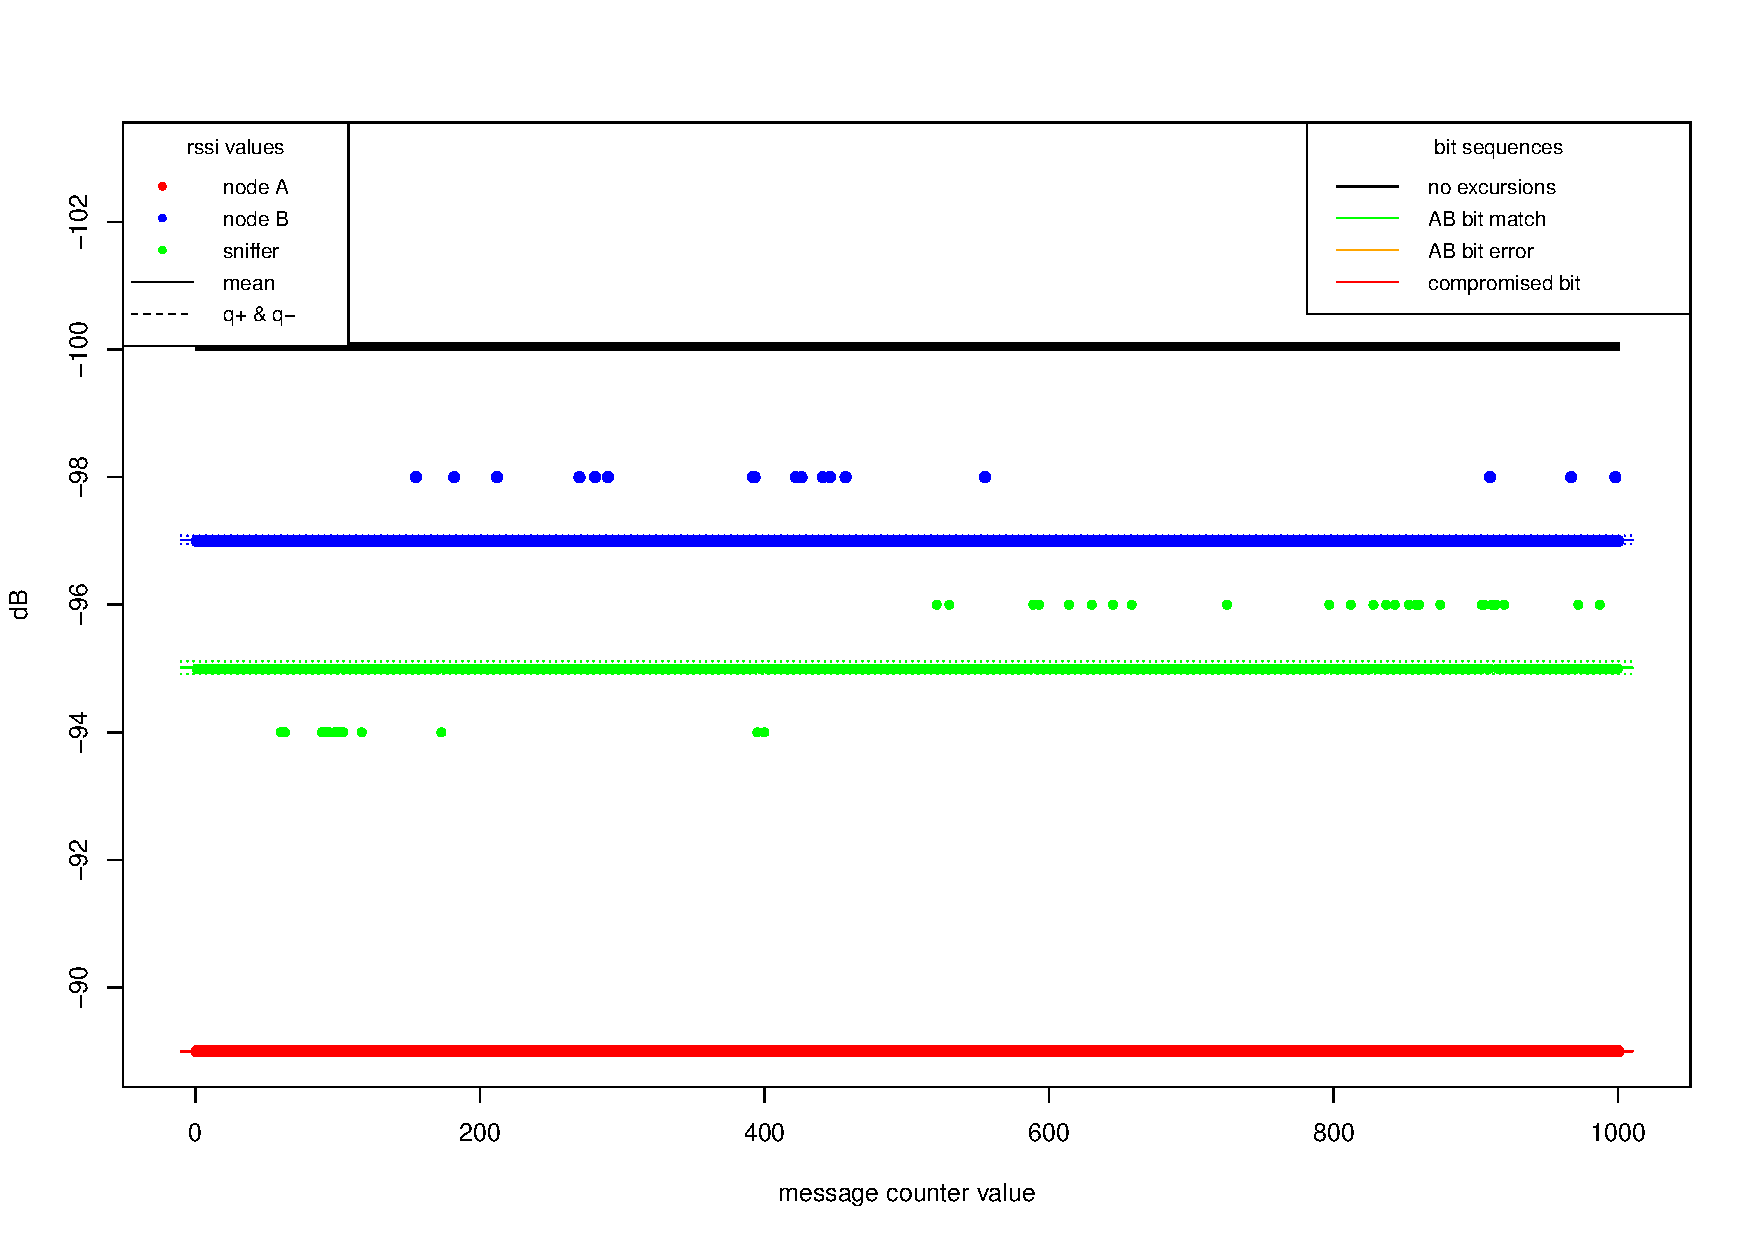
\includegraphics[height=0.9\textwidth, angle = 90 ]{../images/graph_rssi_01.pdf}
\caption{sd = 0}
\label{fig:rssi_01}
\end{figure}

\begin{figure}
  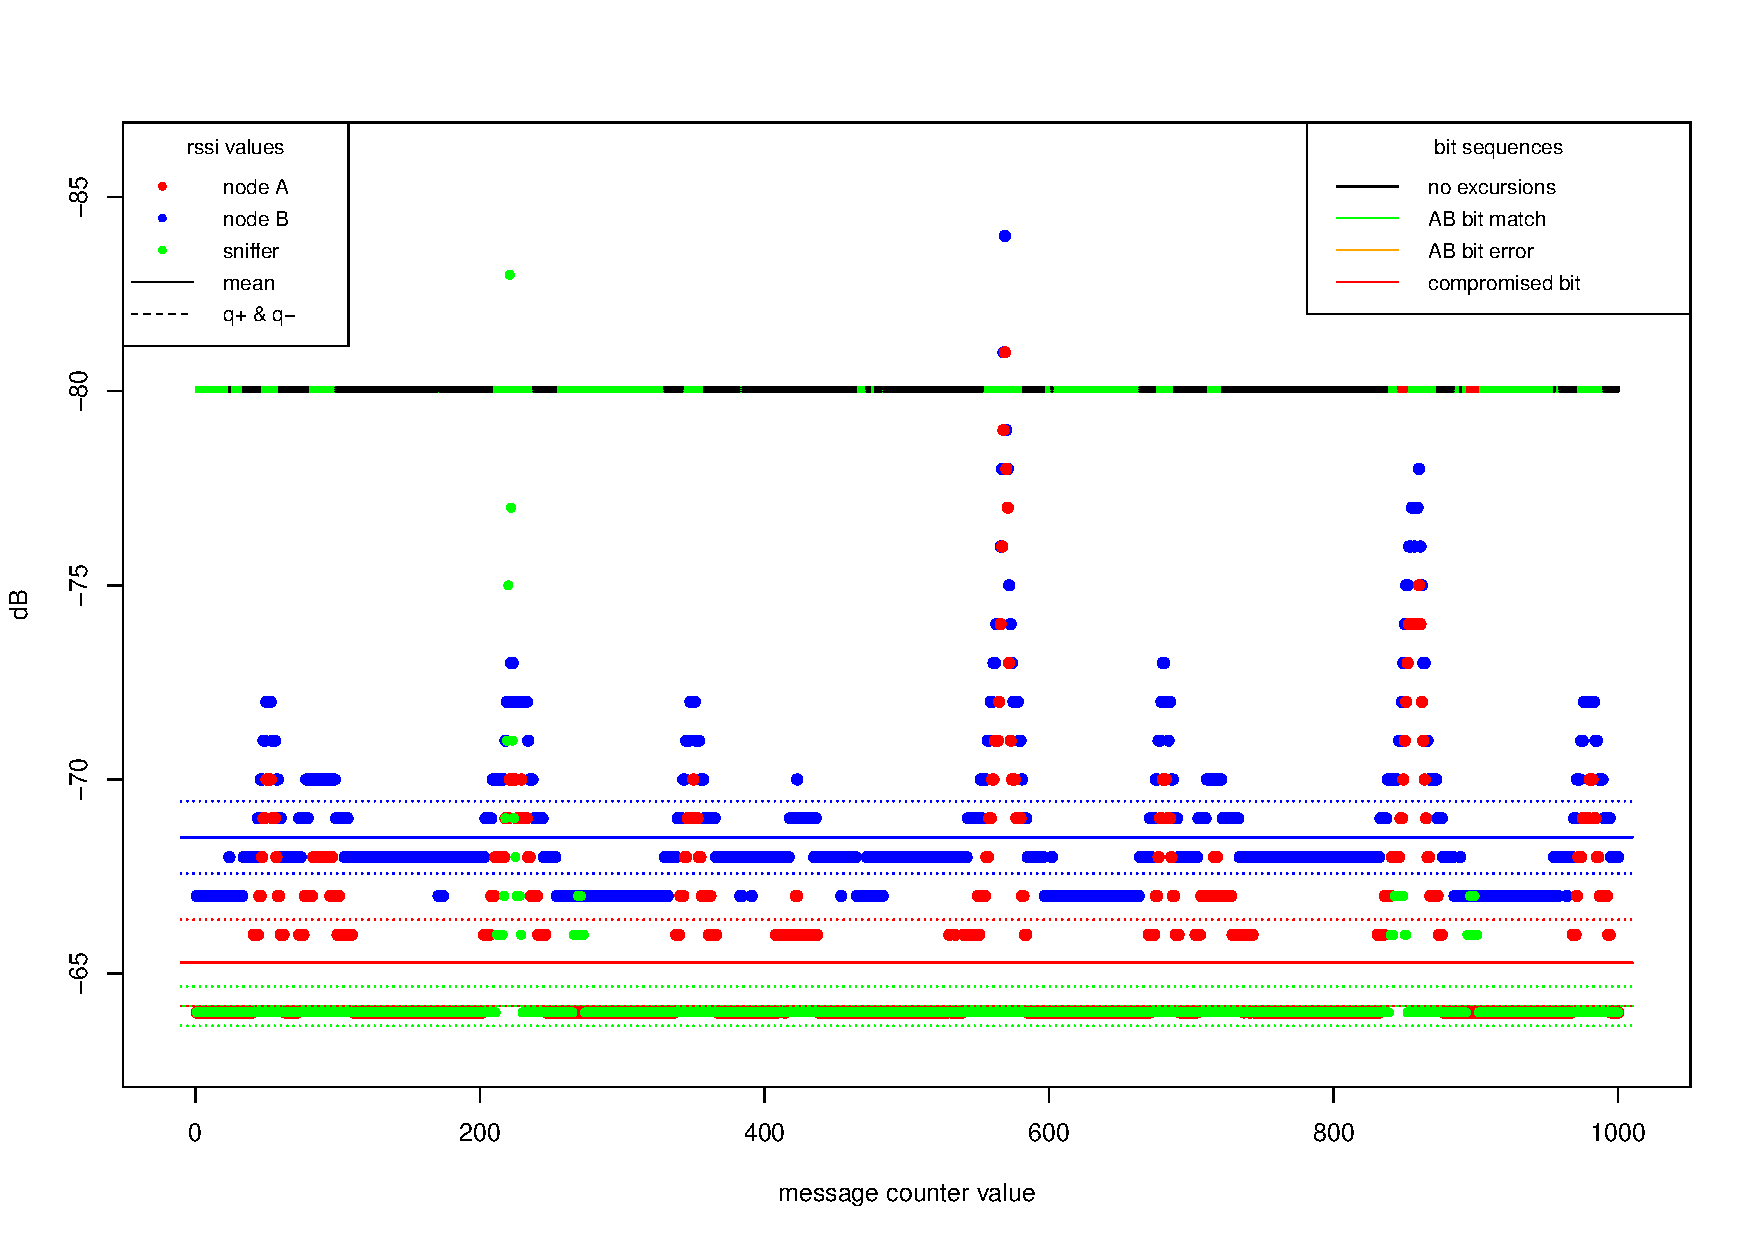
\includegraphics[height=\textwidth, angle = 90 ]{../images/graph_rssi_02.pdf}
\caption{spikes}
\label{fig:rssi_02}
\end{figure}

\begin{figure}
  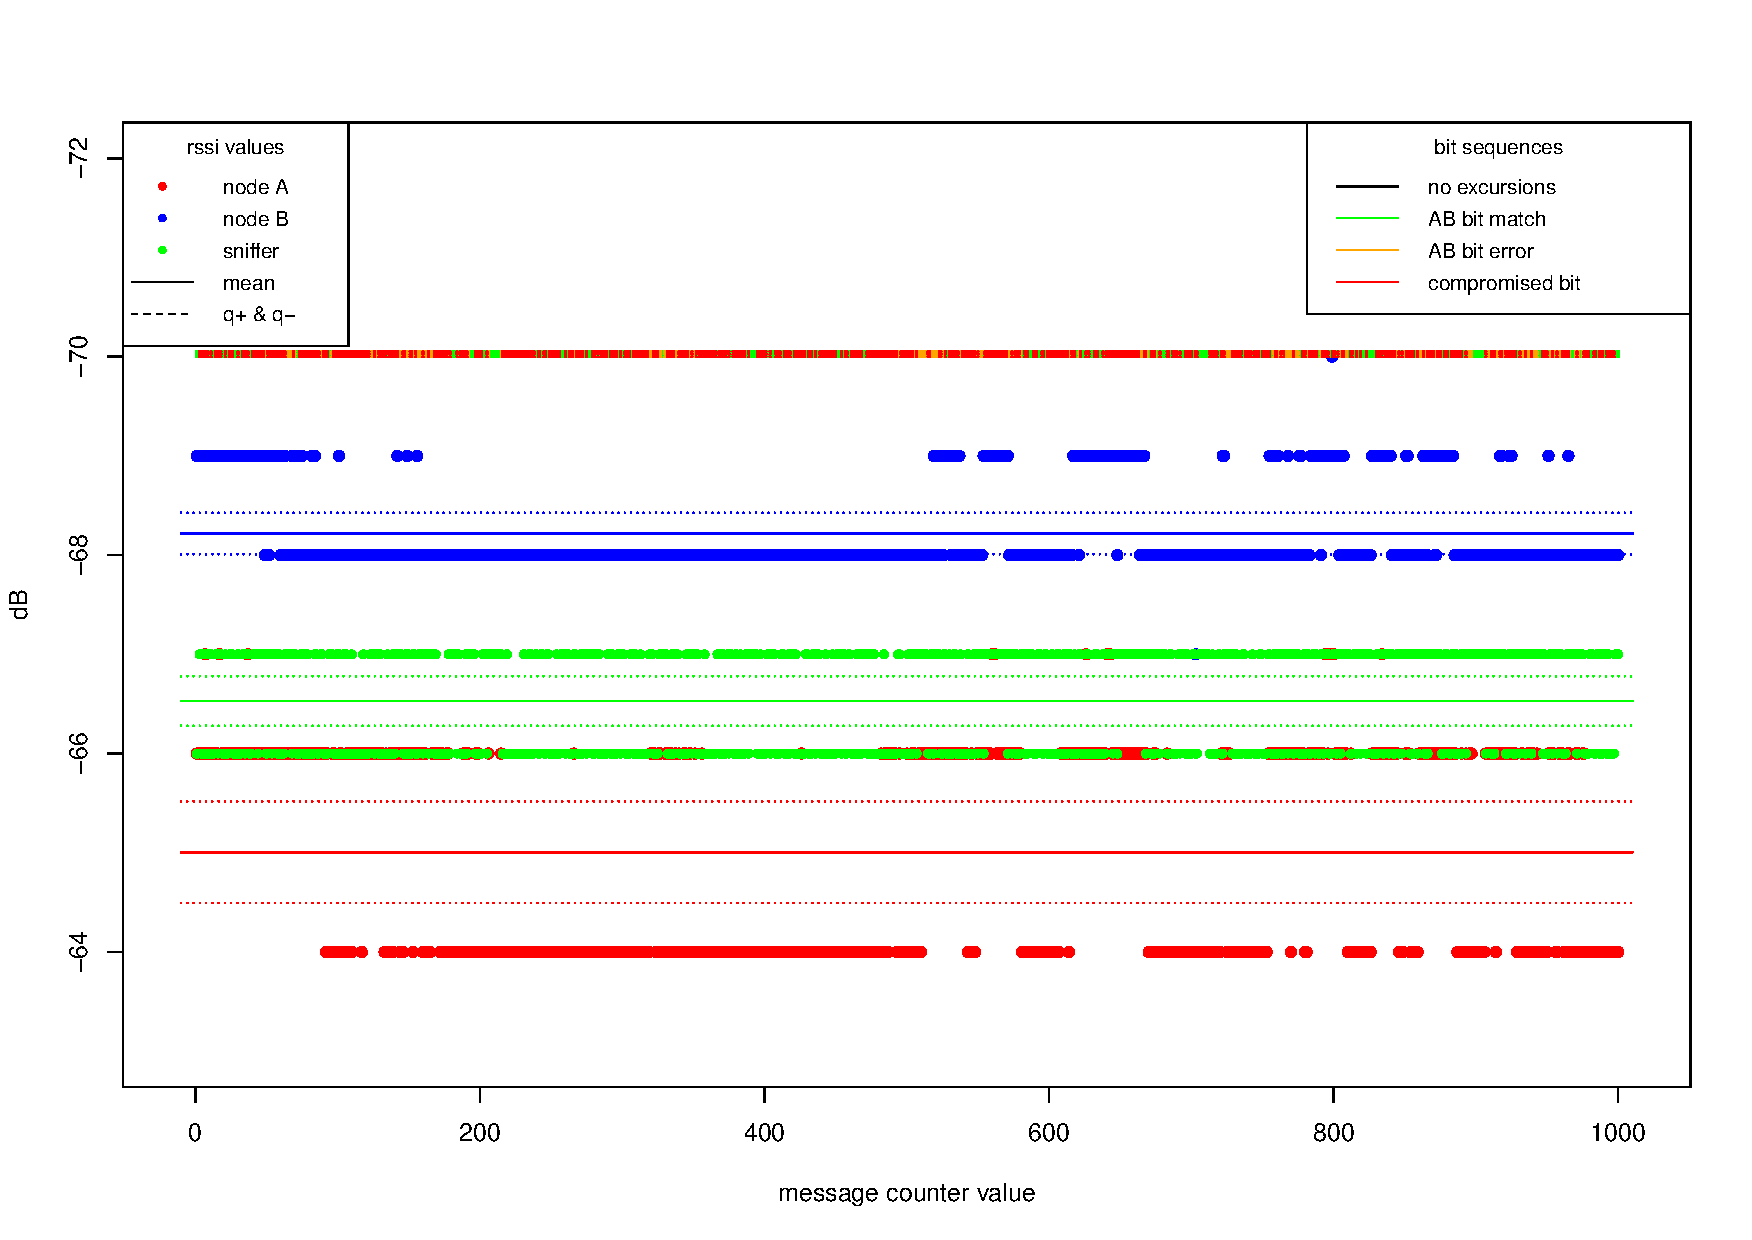
\includegraphics[height=\textwidth, angle = 90 ]{../images/graph_rssi_03.pdf}
\caption{1000 bits output}
\label{fig:rssi_03}
\end{figure}

\end{document}
